\documentclass[a4paper, 11pt, oneside, openright, english]{book}
\usepackage[utf8]{inputenc}
\usepackage{graphicx}
\usepackage{hyperref}
\usepackage{booktabs}
\usepackage{blindtext}
\usepackage{amsmath}
\usepackage{amssymb}
\usepackage{listings}
\usepackage{titlesec}
\usepackage{longtable}
\usepackage{seqsplit}
\usepackage{geometry}
\usepackage{fancyhdr}
\usepackage{float}
\usepackage{enumitem}
\usepackage{array}
\usepackage{multicol}
\usepackage{caption}
\usepackage{listings}
\usepackage[T1]{fontenc}  % Use T1 font encoding
\usepackage{beramono}
\usepackage[dvipsnames]{xcolor}

\pagestyle{fancy}
\fancyhf{}

\fancyhead[LE,RO]{\slshape \rightmark}
\fancyhead[LO,RE]{\slshape \leftmark}
\fancyfoot[C]{\thepage}
\renewcommand{\chaptermark}[1]{\markboth{#1}{}}
\renewcommand{\sectionmark}[1]{\markright{\thesection.\ #1}}

\setlength{\headheight}{13.59999pt}
\addtolength{\topmargin}{-1.59999pt}

\titleformat{\chapter}[block]{\normalfont\huge\bfseries}{\thechapter.}{1em}{\Huge}

\begin{document}
\input title
\input revision_history
\tableofcontents

\chapter{Introduction}

\section{Purpose}
The purpose of this document is to present a detailed description of CodeKataBattle (CKB).
It provides functional and non-functional requirements for the development of the system, including use cases, features, user interaction and system constraints. This document is addressed to the developers who have to implement the requirements and
could be used as an agreement between the customer and the contractors.

CodeKataBattle (CKB) is a new platform that helps students improve their software development skills by training with peers on code kata. Educators use the platform to challenge students by creating code
kata battles in which teams of students can compete against each other, thus proving (and improving) their skills and soft-skills : in fact working in a team is useful to learn soft-skills such as
communication and coordination.

A code kata battle is essentially a programming exercise in a programming language of choice (e.g.,
Java, Python). The exercise includes a brief textual description and a software project with build
automation scripts (e.g., a Gradle project in case of Java sources) that contains a set of test cases that
the program must pass, but without the program implementation. Students are asked to complete the
project with their code. In particular, groups of students participating in a battle are expected to follow
a test-first approach and develop a solution that passes the required tests. Groups deliver their
solution to the platform (by the end of the battle). At the end of the battle, the platform assigns scores
to groups to create a competition rank.

\subsection{Goals}
% \par\noindent\rule{
% \begin{table}[h]
%     \begin{tabular}{ c p{2cm} }
%         \hline
%         \textbf{G1} & Allows Students to improve their software development skills by partecipating in coding tournaments where they write programs \\
%         \textbf{G2} & Allows Educators to challenge Students by create coding tournaments and battles.                                              \\
%         \hline
%     \end{tabular}
%     \label{tab:Goals}
% \end{table}
% }

\begin{description}
    \item \textbf{G1} \quad Allows Students to improve their software development skills by partecipating in coding tournaments where they write programs
    \item \textbf{G2} \quad Allows Educators to challenge Students by create coding tournaments and battles.
    \item \textbf{Gi} \quad Allows Educators to track Students' knowledge about software development, evaluating the code written during battles and the overall score obtained in tournaments
    \item \textbf{Gi} \quad Allows Educators to customize battles defining specific rules, achivements that Students can obtain and evaluation modality.
    \item \textbf{Gi} \quad Allows Students to improve their soft skills, as communication, collaboration and time management, by creating teams for coding battles
    \item {\textcolor{red}{Non son sicuro siano goal che Code kata vuole risolvere}}
    \item \(G_i\) Allows S to learn sw develoment divertendosi e confrontandosi con i compagni in sane competizioni con ranking
\end{description}
\par\noindent\rule{\textwidth}{0.5pt}

\blindtext
\section{Scope}

{\color{red} In another RASD here there are a few words}

\subsection{World Phenomena}
\par\noindent\rule{\textwidth}{0.5pt}
\begin{description}
    \item \textbf{WP1} \quad The students fork the GitHub repository of the code kata
    \item \textbf{WP1} \quad Students set up an automatic workflow in the GitHub repository
    \item \textbf{WP1} \quad The students work on the code kata battle
    \item \textbf{WP1} \quad The students push their work to the GitHub repository
    \item \textbf{WP1} \quad An educator upload correct test cases and automation scripts
    \item \textbf{WP1} \quad An educator evaluates the work done by the team at the end of the code kata battle
\end{description}
\par\noindent\rule{\textwidth}{0.5pt}


\subsection{Shared Phenomena}
\begin{description}
    \item \(SP_i\) An educator creates a tournament
    \item \(SP_i\) An educator grants other colleagues permission to create battles
    \item \(SP_i\) An educator creates a battle within a tournament
    \item \(SP_i\) The students are notified of a new tournament
    \item \(SP_i\) The students are notified of a new upcoming battle within a tournament they are subscribed to
    \item \(SP_i\) Students use the platform to form teams
    \item \(SP_i\) Student invite other students to join its team respecting the boundaries imposed
    \item \(SP_i\) Student join a battle on his own
    \item \(SP_i\) Student join a battle towards an invite -> Possono scegliere di essere soli oppure devono per forza
    \item \(SP_i\) The platform sends the link of the GitHub repository to all students who are members of subscribed teams
    \item \(SP_i\) Students are asked to fork the GitHub repository and set up an automated workflow
    \item \(SP_i\) The forked repository's workflow notifies the platform of a new push
    \item \(SP_i\) The platform updates the battle score of a team
    \item \(SP_i\) The educator uses the platform to go through the sources produced by each team
    \item \(SP_i\) The educator assigns additional score to the teams after the evaluation
    \item \(SP_i\) The platform notifies the teams when the final battle rank becomes available
    \item \(SP_i\) The platform updates the personal tournament score of each student
    \item \(SP_i\) An educator closes a tournament
    \item \(SP_i\) The platform notifies all students involved in the tournament about its end
    \item \(SP_i\) All users see the list of  ongoing tournaments as well as the corresponding tournament rank
    \item \(SP_i\) An educator defines the gamification badges
    \item \(SP_i\) Student visualize gained badges on its profile
\end{description}

\section{Definitions, Acronyms, Abbreviations}
\subsection{Abbreviations}
\(G_i\) = i-th goal \\
\(WP_i\) = i-th World Phenomena\\
\(SP_i\) = i-th Shared Phenomena\\

\subsection{Acronyms}
E = educator \\
S = students
\section{Revision history}
\section{Reference Documents}
Assign document for A.Y. 2023-2024 "Requirement Engineering and Design Project: goal, schedule, and rules"

\section{Document Structure}
The structure of this RASD document follows six main sections:
\begin{enumerate}
    \item \textbf{Introduction:}
          provides an overview of the problem at hand, the purpose of the document and
          the project, the scope of the domain, and introduces the main goals of the system as a solution.

    \item \textbf{Overall Description:}
          gives a general description of the system, going into more details about its main functions.
          The description is assisted with the help of UML diagrams, such as class, activity and state diagram.
          The domain assumptions of the examined world are then explained along with any dependencies and constraints.

    \item \textbf{Specific Requirements:}
          

    \item \textbf{Formal Analysis Using Alloy:}

    \item \textbf{Effort Spent:}
          keeps track of the time spent to complete this document.
          The first table defines the amount of hours used by the whole team to get important decisions and to make reviews,
          the other tables contains the individual effort spent by each team member.

    \item \textbf{References:}
          lists all the documents used and that were helpfull in drafting the RASD.
\end{enumerate}
\chapter{Architectural Design}

\section{Overview}
The CKB platform system is composed by a 3-tier architecture.\\
Its software application architecture is organized into three logical tiers: the presentation tier, or user interface; the application tier, where data is processed; and the data tier, where the data associated with the application is stored and managed.

\begin{figure}[H]
    \centering
    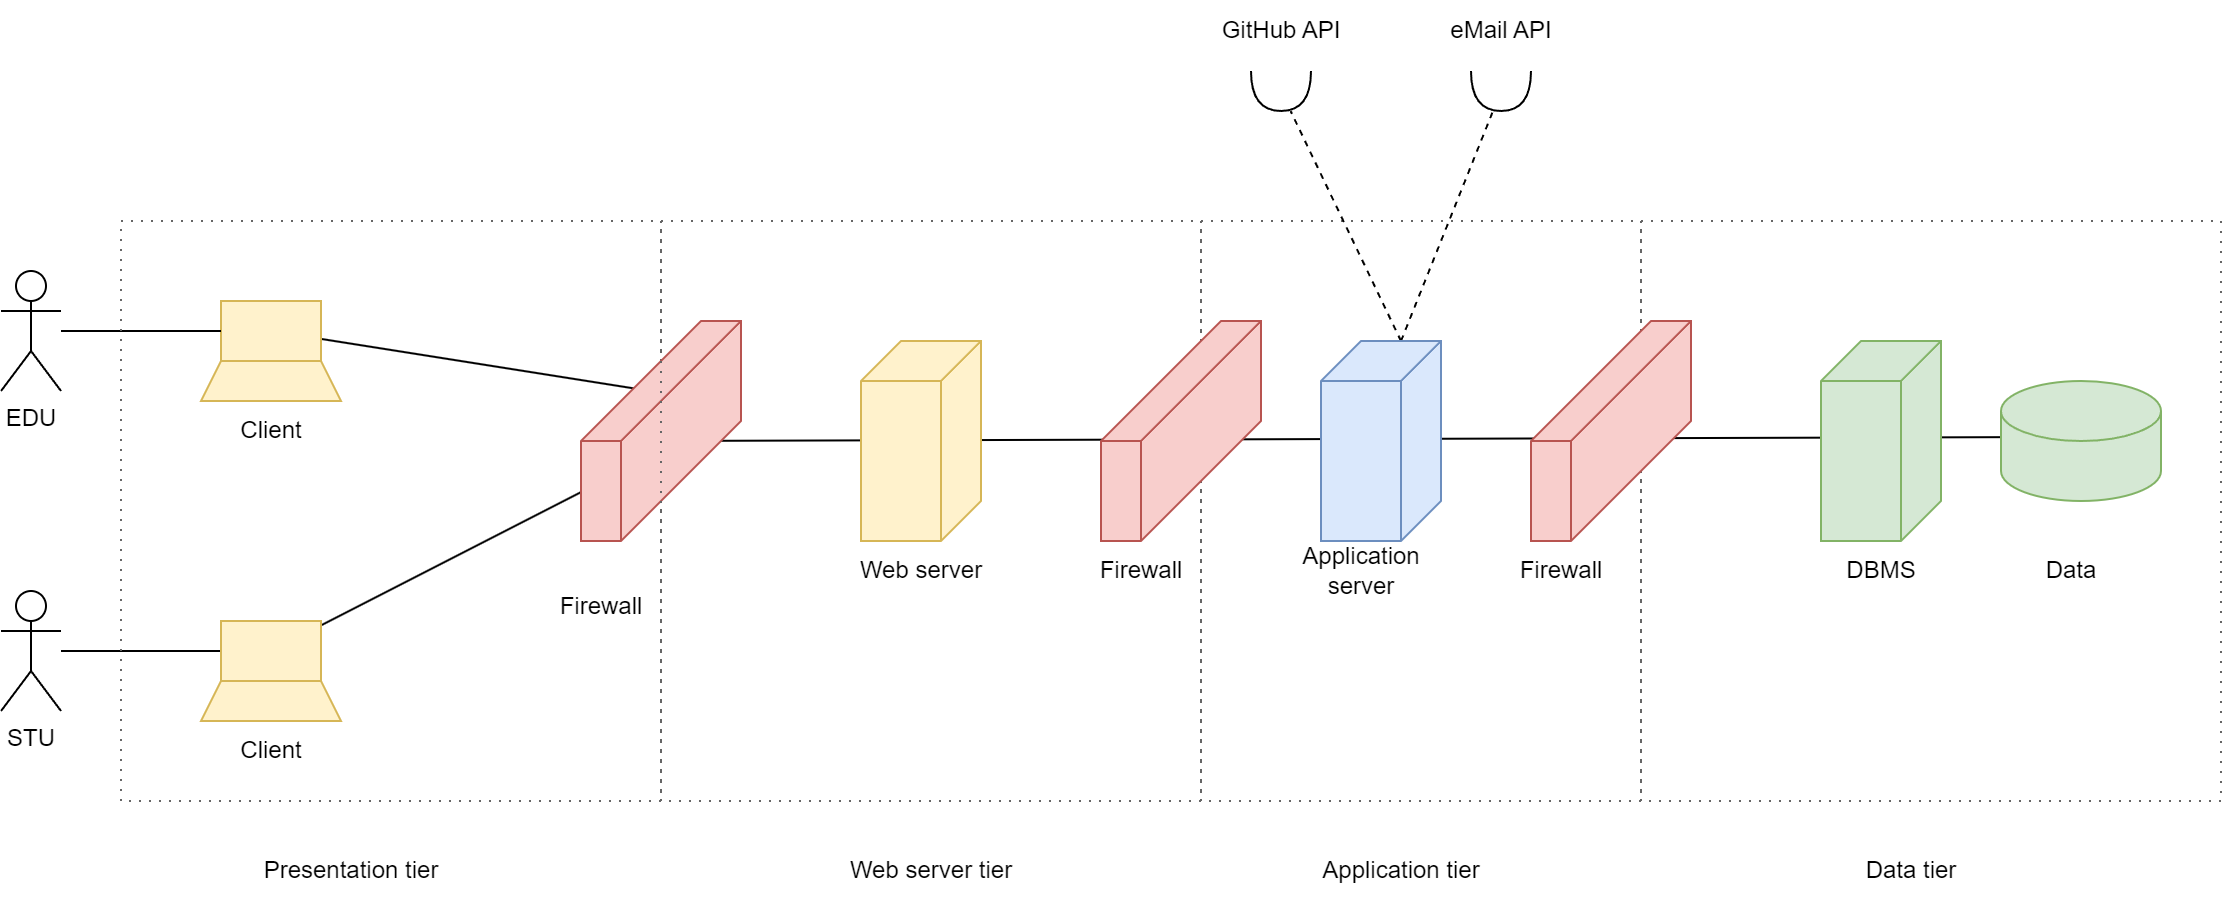
\includegraphics[width=\textwidth]{images/diagrams/high_level_diagram.png}
    \caption{High level components diagram}
\end{figure}

The service will be accessed through a web interface, employing a Single Page Application (SPA). Utilizing an SPA is ideal for this application, as it facilitates extensive interaction without necessitating frequent page reloads.\\
The system's architecture is structured into distinct layers, with application servers interacting with a database management system and utilizing APIs for data retrieval and storage. Adhering to REST standards, the application servers are intentionally designed to be stateless, handling the login sessions for user thanks to the caching, following the best practices for web applications.\\
The system will include more than one firewall to ensure security.\\

\section{Component view}
The system is composed by the following components:

\begin{figure}[H]
    \centering
    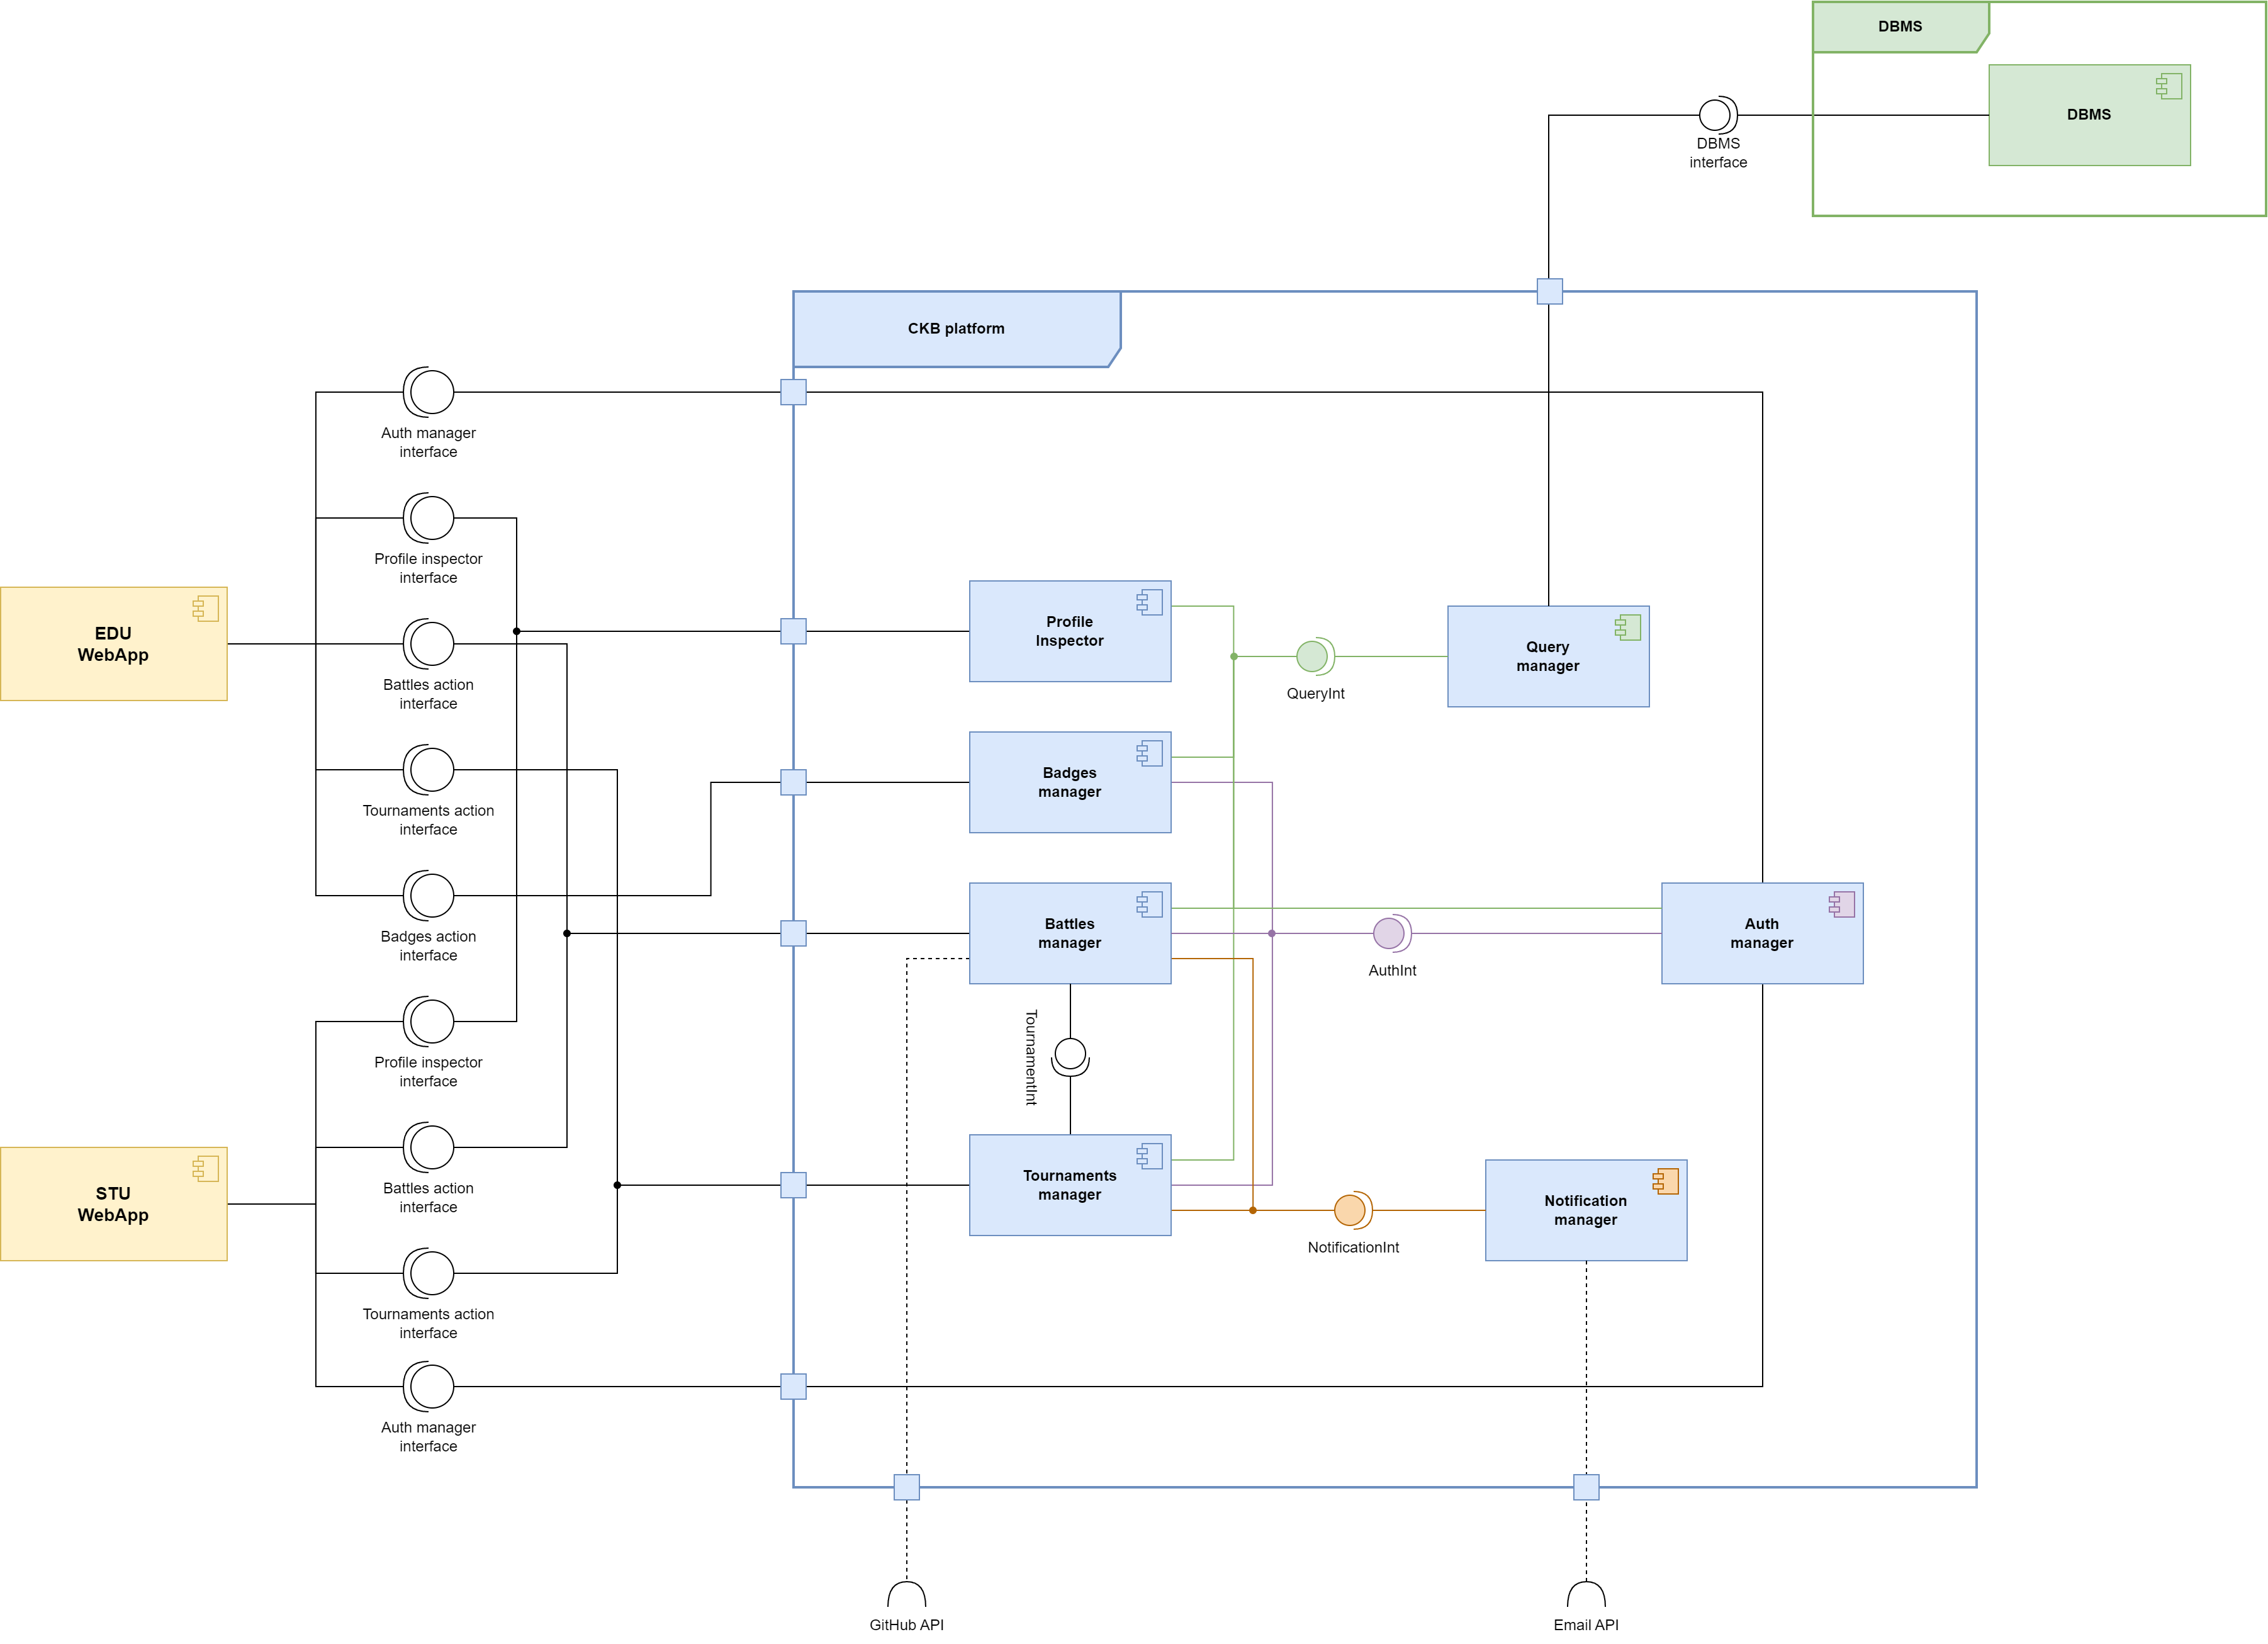
\includegraphics[width=\textwidth]{images/diagrams/component_diagram.png}
    \caption{Component diagram}
\end{figure}

In order to maintain the readability of the diagram, the interfaces have been grouped with respect to their functionality; the complete set of endpoints is available later in the document.\\

\subsection{Client components}

The client components are represented by only a single component, a user-friendly WebApp, that will behave differently depending on the type of the user that is using it (whether it is an EDU or a STU).\\
The WebApp is interfaced with the server components through all the APIs offeded by the server (see later for a detailed description of the APIs).\\

\subsection{Server components}

\subsubsection*{Query manager}
The query manager is the component that handles the queries made by the other components that need to access the database. It is responsible for the execution of the queries and for the communication with the database.\\
It is interfaced with all the internal models of the system that need to access the database, i.e. all the other components of the system exept for the notification manager.\\
It is interfaced with the database through the DBMS API, external to the system.

\subsubsection*{Auth manager}
The auth manager is the component that handles the authentication of the users and the authorization of the requests made by the other components that need to access the database with respect to the user that made the request.\\
It is interfaced with all the internal models of the system that behave differently depending on the level of the user that made the request, i.e. the badges manager, the tournament manager and the battle manager.\\
It isn't interfaced with any external component.

\subsubsection*{Notification manager}
The notification manager is the component that handles the need of the system to notify the users of some events, such as the start of a tournament or the end of a battle.\\
It is interfaced with all the internal models of the system that need to notify the users, i.e. the tournament manager and the battle manager.\\
It is interfaced with the Email API, external to the system.

\subsubsection*{Badges manager}
The badges manager is the component that handles the gamification badges.\\
It allows:
\begin{itemize}
    \item the creation of new badges;
    \item the assignment of badges to the STUs;
    \item the visualization of the badges assigned to a user (?)
\end{itemize}
{\color{red}Qui devo interfacciare anche con battle e user?}
It is interfaced with the auth manager (since the creation of a badge is admissible only for the EDUs) and with the query manager (since it needs to access the database to store the badges).\\
It is interfaced with the EDU WebApp through the proprer, external to the system.

\subsubsection*{Tournaments manager}
The tournament manager is the component that handles the management of the tournaments.\\
It allows:
\begin{itemize}
    \item the creation of new tournaments;
    \item the closure of the torunaments
    \item the visualization of the tournaments;
    \item the excange of admin permission between EDUs;
    \item the subscription of the STUs to the tournaments;
    \item the visualization of the scores of the EDUs in the tournaments, and so of the ranking
\end{itemize}
It is interfaced with the auth manager (to allow and perform different actions depending on the level of the user that made the request), with the query manager (since it needs to access the database) and the notification manager (since it needs to notify the users of the start and the end of a tournament).\\
It is interfaced with the WebApp, both EDU and STU, through the proper APIs, external to the system.

\subsubsection*{Battles manager}
{\color{red} specificare meglio}
The battles manager is the component that handles the management of the battles.\\
It allows:
\begin{itemize}
    \item the creation of new battles;
    \item the subscription of the STUs to the battles;
    \item the visualization of the scores of the teams in the battles, and so of the ranking
    \item the visualization of the battles;
    \item the automatic evaluation of the battles;
    \item the eventual manual evaluation of the battles by the EDUs
\end{itemize}
It is interfaced with the auth manager (to allow and perform different actions depending on the level of the user that made the request), with the query manager (since it needs to access the database) and the notification manager (since it needs to notify the users of the opening of subscriptions, the start and the end of a bettle).\\
It is interfaced with the WebApp, both EDU and STU, through the proper APIs and with GitHub (to perform the manual evaluation), all external to the system.

\subsubsection*{Profile Inspector}
The profile inspector is the component that handles the visualization of the profiles of the STUs and, consequently, of the badges that a STU has earned during the battles and the tournaments.\\
It is interfaced with the query manager (since it needs to access the database).
It is interfaced with the WebApp, both EDU and STU, through the proper APIs, external to the system.

\subsection{Logical description of the data}
The data of the system is organized in a relational database, with the following entity-relationship diagram:

\begin{figure}[H]
    \centering
    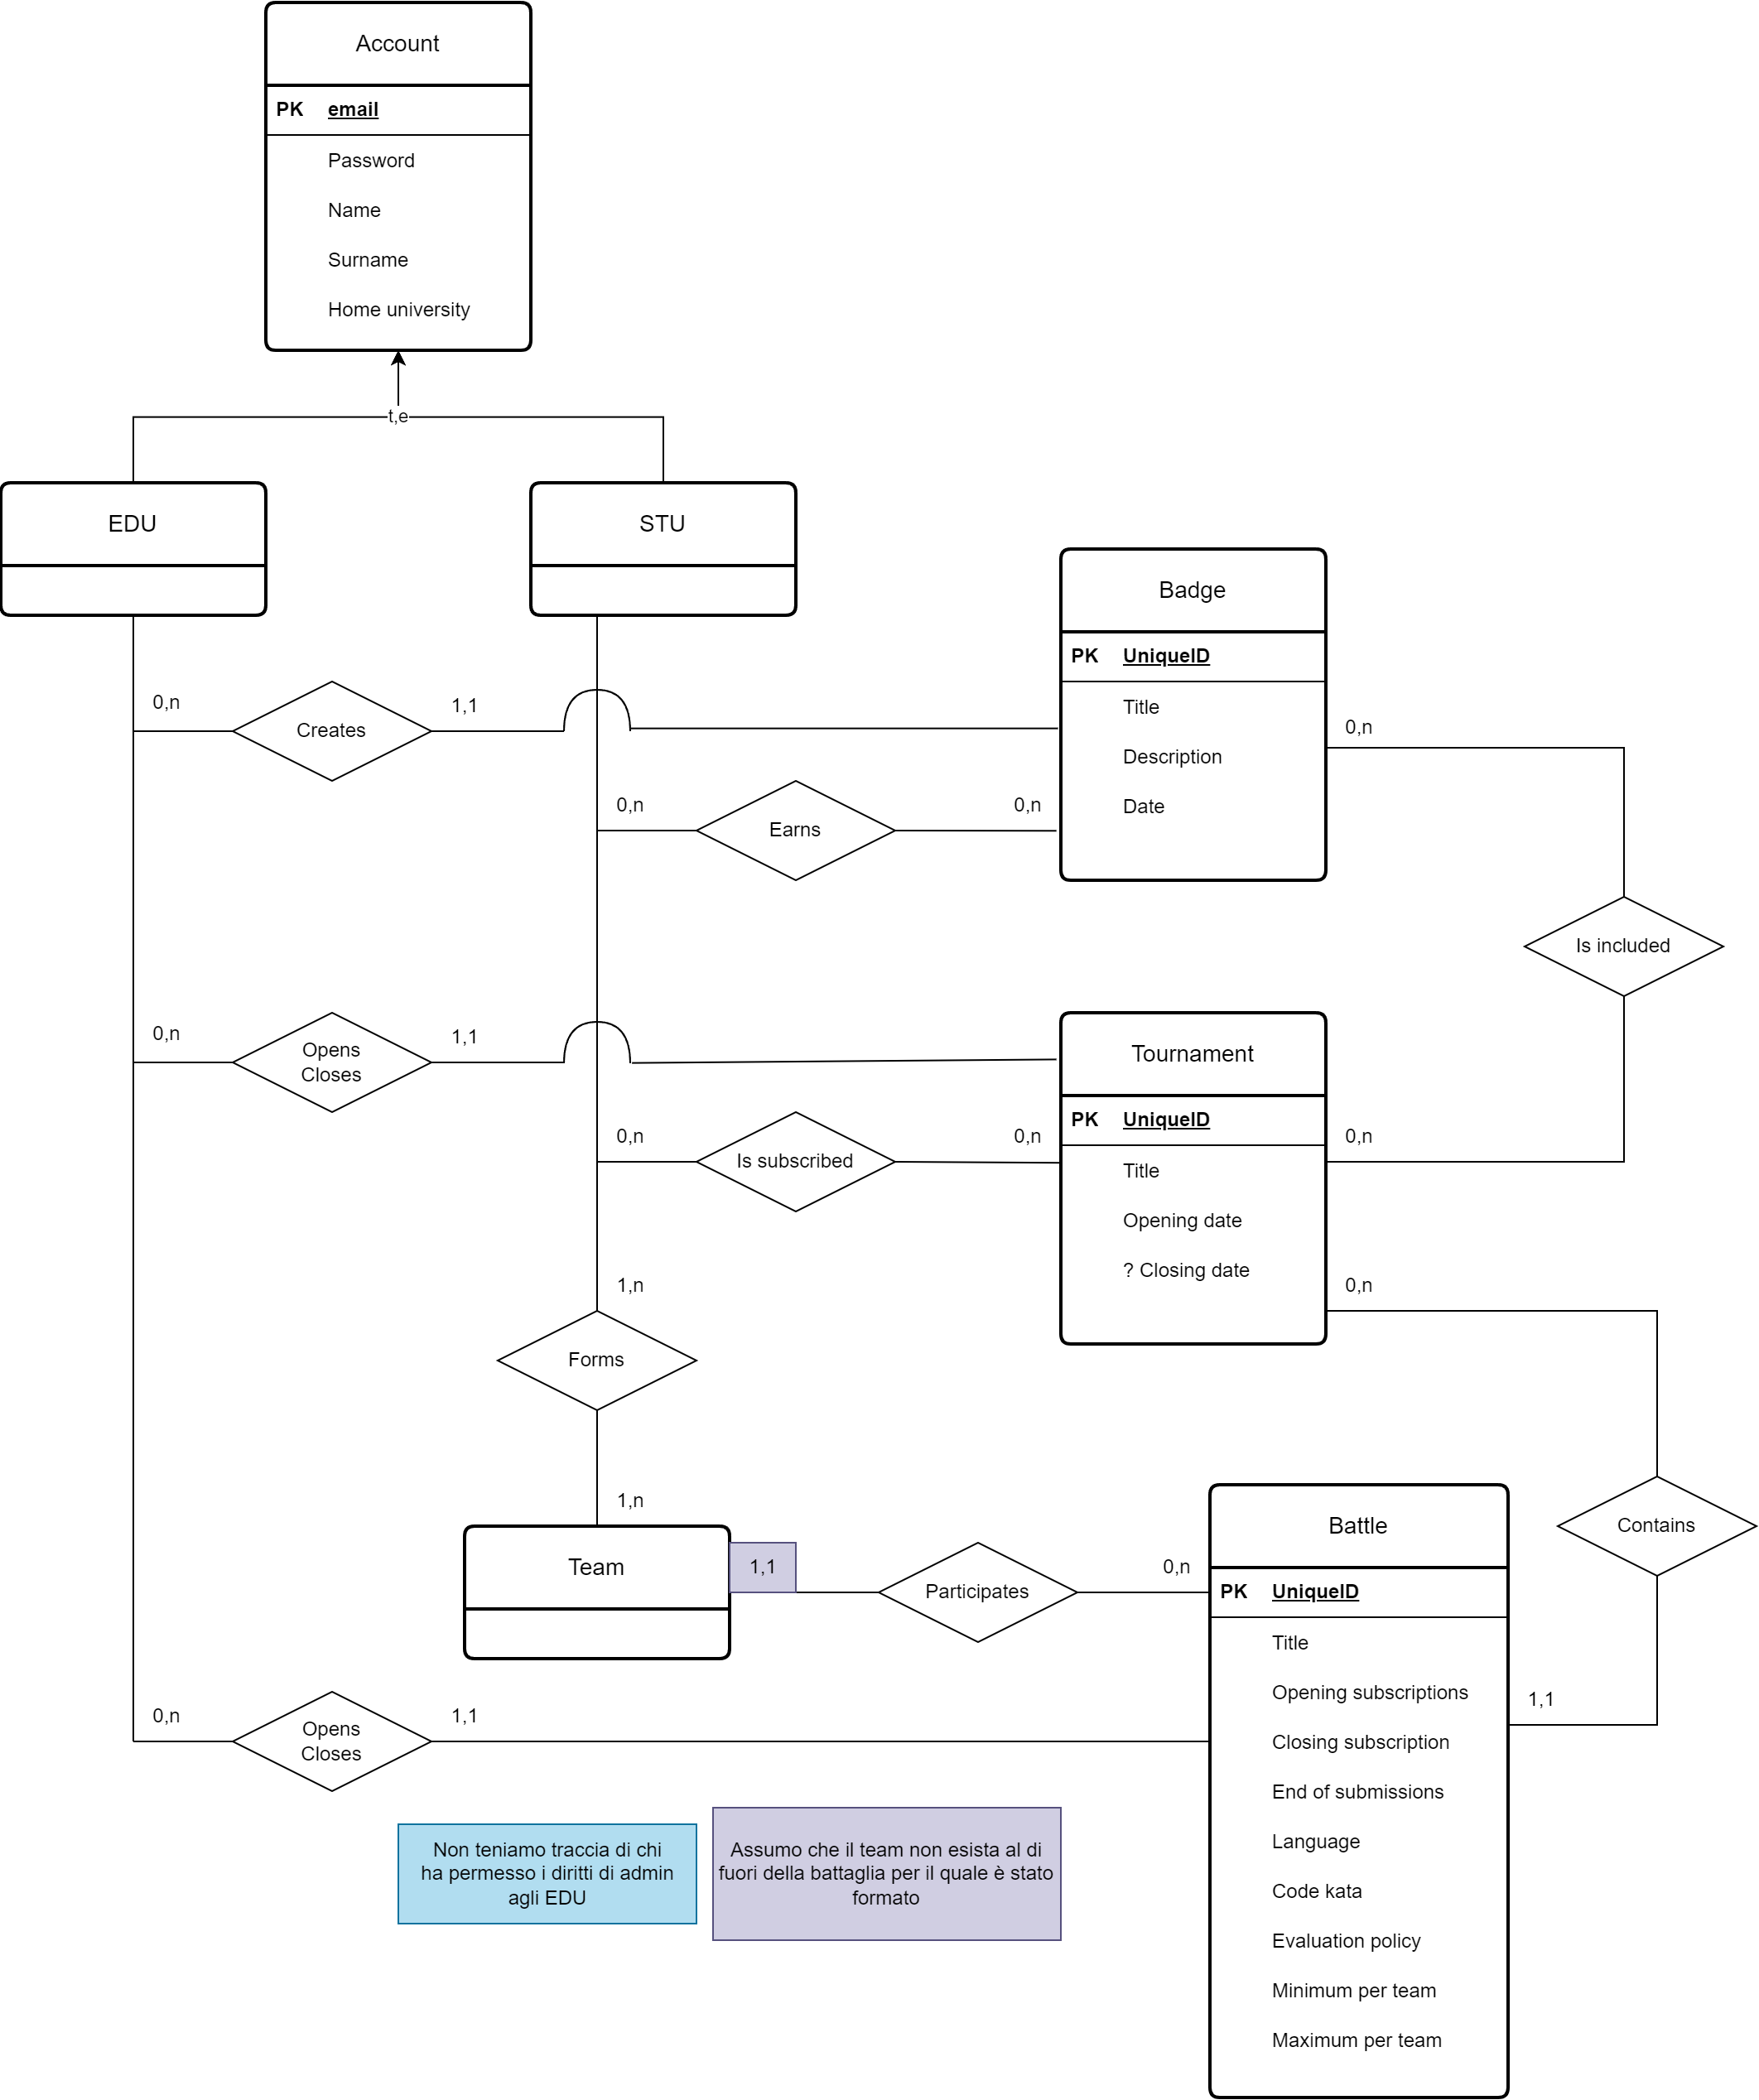
\includegraphics[width=0.75\textwidth]{images/diagrams/er_diagram.png}
    \caption{Entity-relationship diagram}
    \label{fig:er_diagram}
\end{figure}

\section{Deployment view}
The diagram \ref{fig:deployment_diagram} shows the deployment view of the system.\\\\
Our system comprises two essential components: a static web server and an application server. The static web server serves as the entry point for clients to access the SPA, while the application server furnishes the necessary APIs for the SPA's functionality. To optimize performance, we have opted for distinct solutions for these components.\\
The static web server will be hosted on a CDN (Content Delivery Network) on cloud, exploiting its edge location caches and reverse proxies to ensure rapid response times. On the other hand, the application server, containing both a business logic layer and a data tier, will find its home on a cloud provider. This decision offers numerous advantages over traditional in-house hosting, including:
\begin{itemize}
    \item \textbf{Scalability and Flexibility}: The cloud infrastructure allows for the dynamic addition or removal of resources like virtual machines, performance cores, or memory as per the evolving needs. Load balancing services further enable the application server to adapt seamlessly to changes in traffic or workload.
    \item \textbf{Security}: Enhanced security features, such as live monitoring and firewalls, contribute to safeguarding the application server against potential data breaches, cyberattacks, and other security threats.
    \item \textbf{Cost-efficiency}: The cloud provider's pay-as-you-go model ensures cost efficiency by charging only for the utilized resources. This approach helps in reducing overall costs, making it a financially prudent choice.
\end{itemize}
These attributes position a cloud provider as an ideal hosting solution for large, high-traffic applications. The selected cloud provider must respect all these features to effectively meet our system requirements.\\

\begin{figure}[ht]
    \centering
    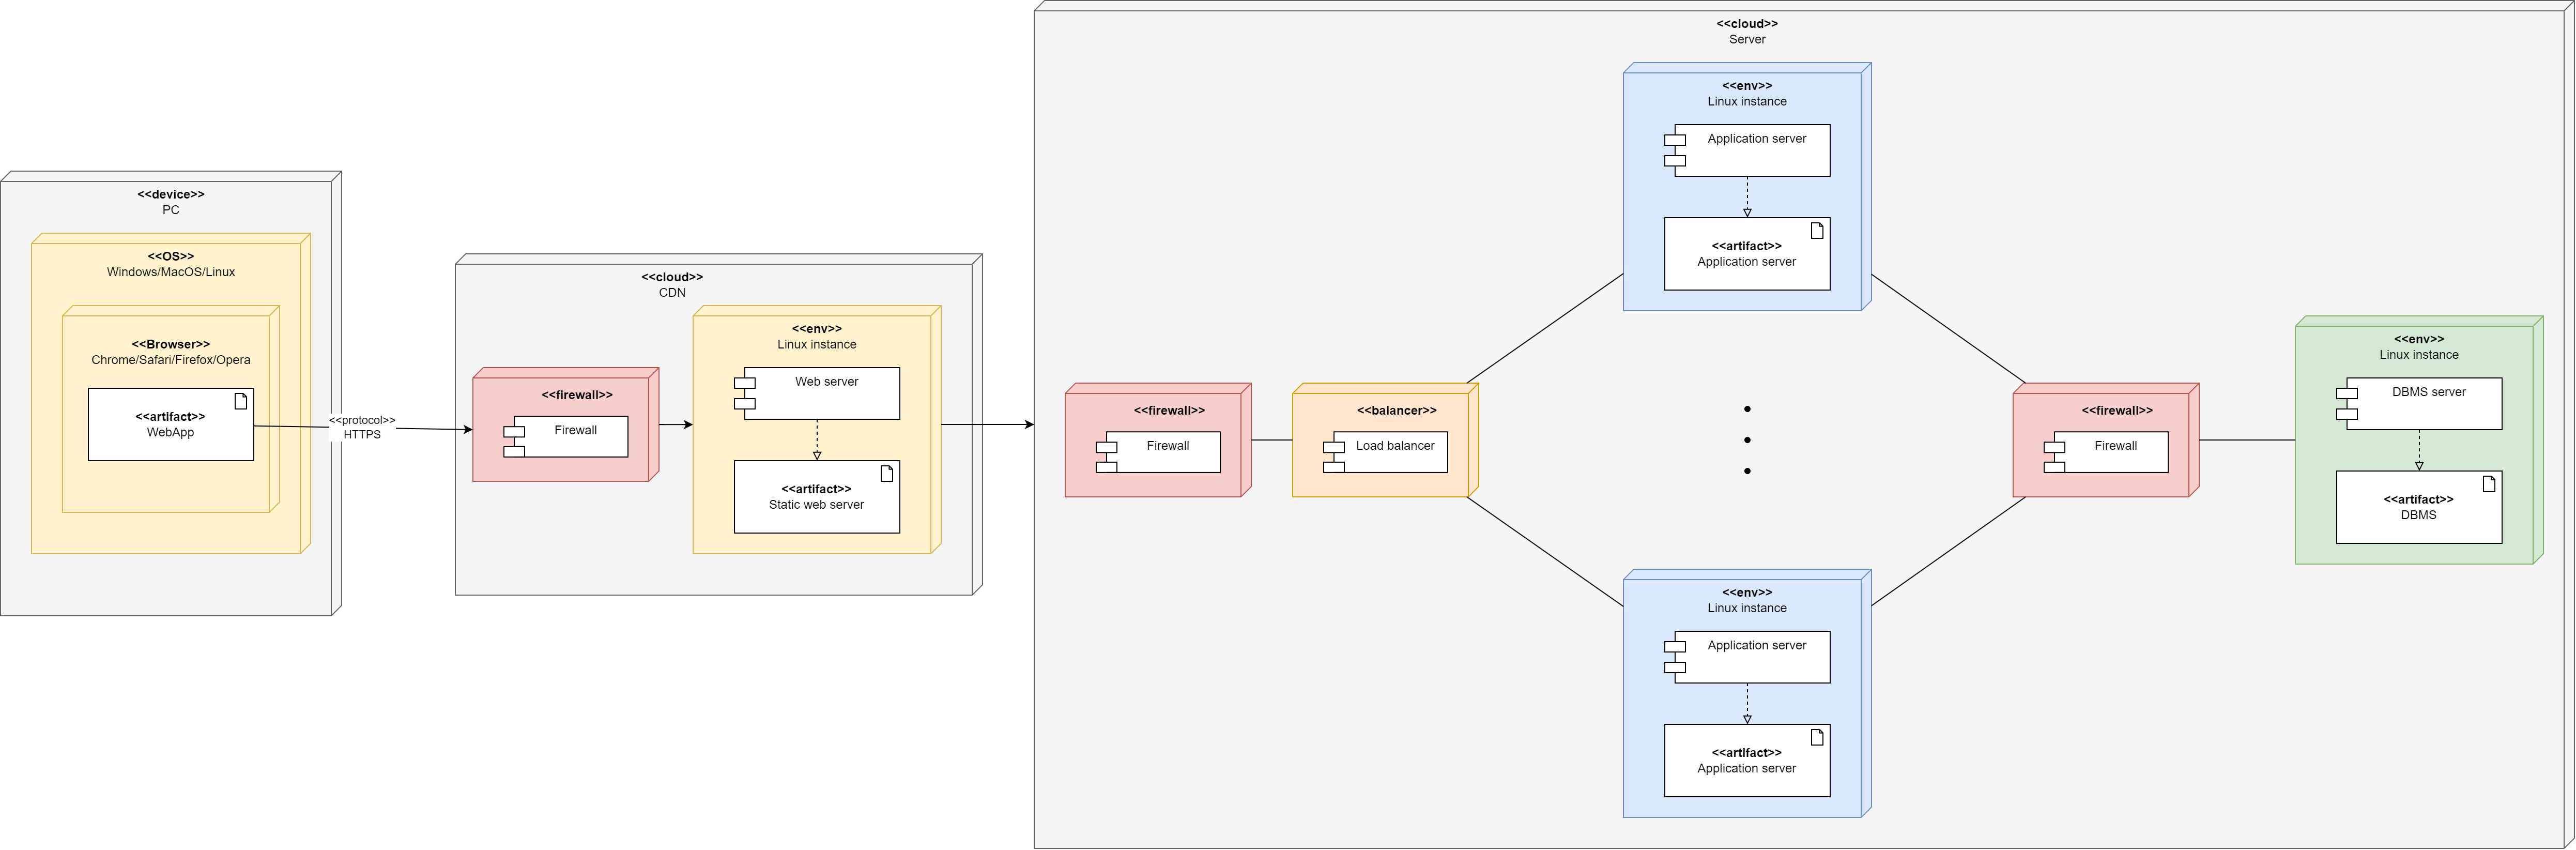
\includegraphics[width=\textwidth]{images/diagrams/deployment_view.png}
    \caption{Deployment diagram}
    \label{fig:deployment_diagram}
\end{figure}

{\color{red} mettere la cdn in mezzo, come sulle slides di tiw}

The components of the system are explaineed in the following:
\begin{itemize}
    \item \textbf{PC}: Personal computer of the user, it suffices to have a wordking O.S. and a browser installed that supports JavaScript and HTML5 in order to use the system.
    \item \textbf{CDN}: As said before, the CDN is used to host the static web server, that serves as the entry point for clients to access the SPA. It will allow it to be downloaded without affecting the performance of the main application server. The SPA is static and all of its code is run on the client's machine, so there is no need for any logic to be implemented on the CDN side.
    \item \textbf{Cloud provider}: The cloud provider is used to host the application server. It will allow the system to be scalable and flexible, to be secure and to be cost-efficient.\\
          It is composed by:
          \begin{itemize}
              \item \textbf{Load balancer}: The load balancer is used to distribute the traffic between the different instances of the application server. It is used to make the system scalable and flexible.
              \item \textbf{Application servers}: The application servers are used to host the application server. They will be in an array of instances, so that the load balancer can distribute the traffic between them. The number of instances can be changed dynamically, so that the system can adapt to the traffic. They are used to make the system scalable and flexible.
              \item \textbf{DBMS server}: The DBMS server is used to host the database.
              \item \textbf{Firewalls}: They are used to make the system secure, and are placed between the load balancer and the external world and between the application servers and the DBMS server. They provide an additional layer of security by blocking or allowing traffic based on predetermined rules. This helps to protect the system from unauthorized access or malicious attacks
          \end{itemize}
\end{itemize}


{\color{red} Da qui in avanti in questo capitolo dobbiamo prima parlarne un secondo su cosa metter (secondo me la sezione \textit{API endpoints}, visto che c'è prevalentemente server-side, dovrebbe scriverlo chi si occuperà del backend )}
\section{Runtime View}
This section describes the most important components interactions of the system.

\subsection{User login}
At the beginning the end user must log in to use the main functions of the application. The login is done by enetring the email and password. If the credentials are present in the database and correct the process will be successful and it will be able to open its dashboard, otherwise it will have to repeat the procedure. (Figure \ref{fig:RuntimeView_UserLogin})
\begin{figure}[H]
    \centering
    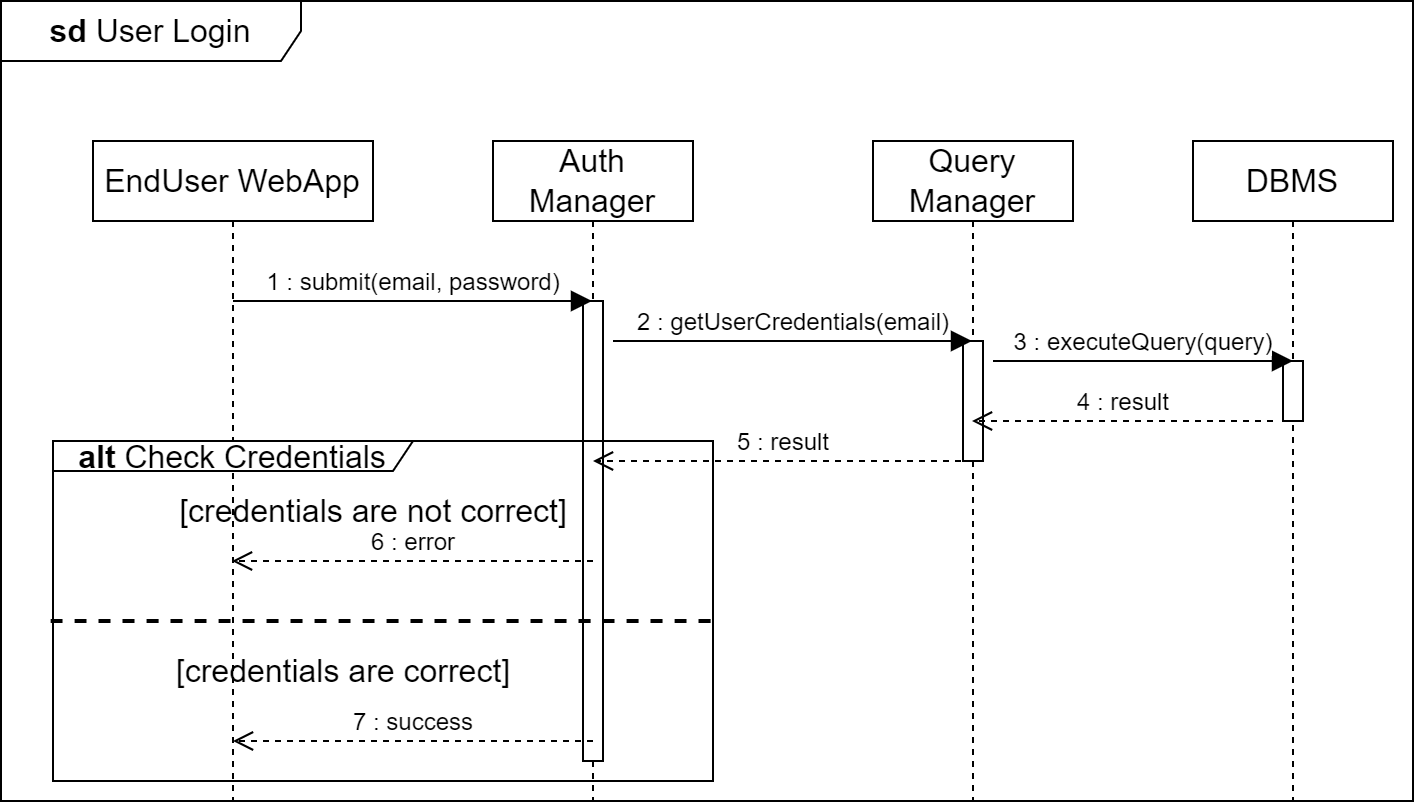
\includegraphics[width=\textwidth]{images/runtimeviews/RuntimeView_UserLogin.png}
    \caption{Runtime View of User Login Event}
    \label{fig:RuntimeView_UserLogin}
\end{figure}

\subsection{Create a tournament}
The following sequence diagram is used to explain how to create a tournament. The end user from its device can create a tournament entering the correlated details through the related component, which are sent to the database. If the tournament has been created successfully, the correlated page is created.(Figure \ref{fig:RuntimeView_CreateTournament} )
\begin{figure}[H]
    \centering
    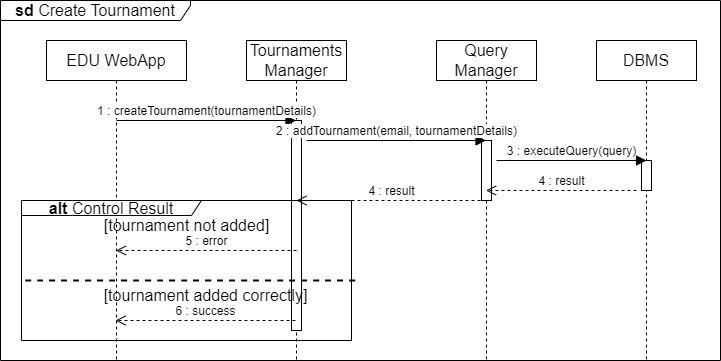
\includegraphics[width=\textwidth]{images/runtimeviews/RuntimeView_CreateTournament.png}
    \caption{Runtime View of Create a Tournament Event}
    \label{fig:RuntimeView_CreateTournament}
\end{figure}

\subsection{Create a battle}
The following sequence diagram is used to explain how to create a battle within a tournament. The end user from its device can create a battle entering the correlated details through the related component. If the user is a granted educator for the current tournament, then the details of the new battle are sent to the database and if the battle has been created successfully, the correlated page is created and all the users subscribed to the correlated tournament are notified. (Figure \ref{fig:RuntimeView_CreateBattle}) 
\begin{figure}[H]
    \centering
    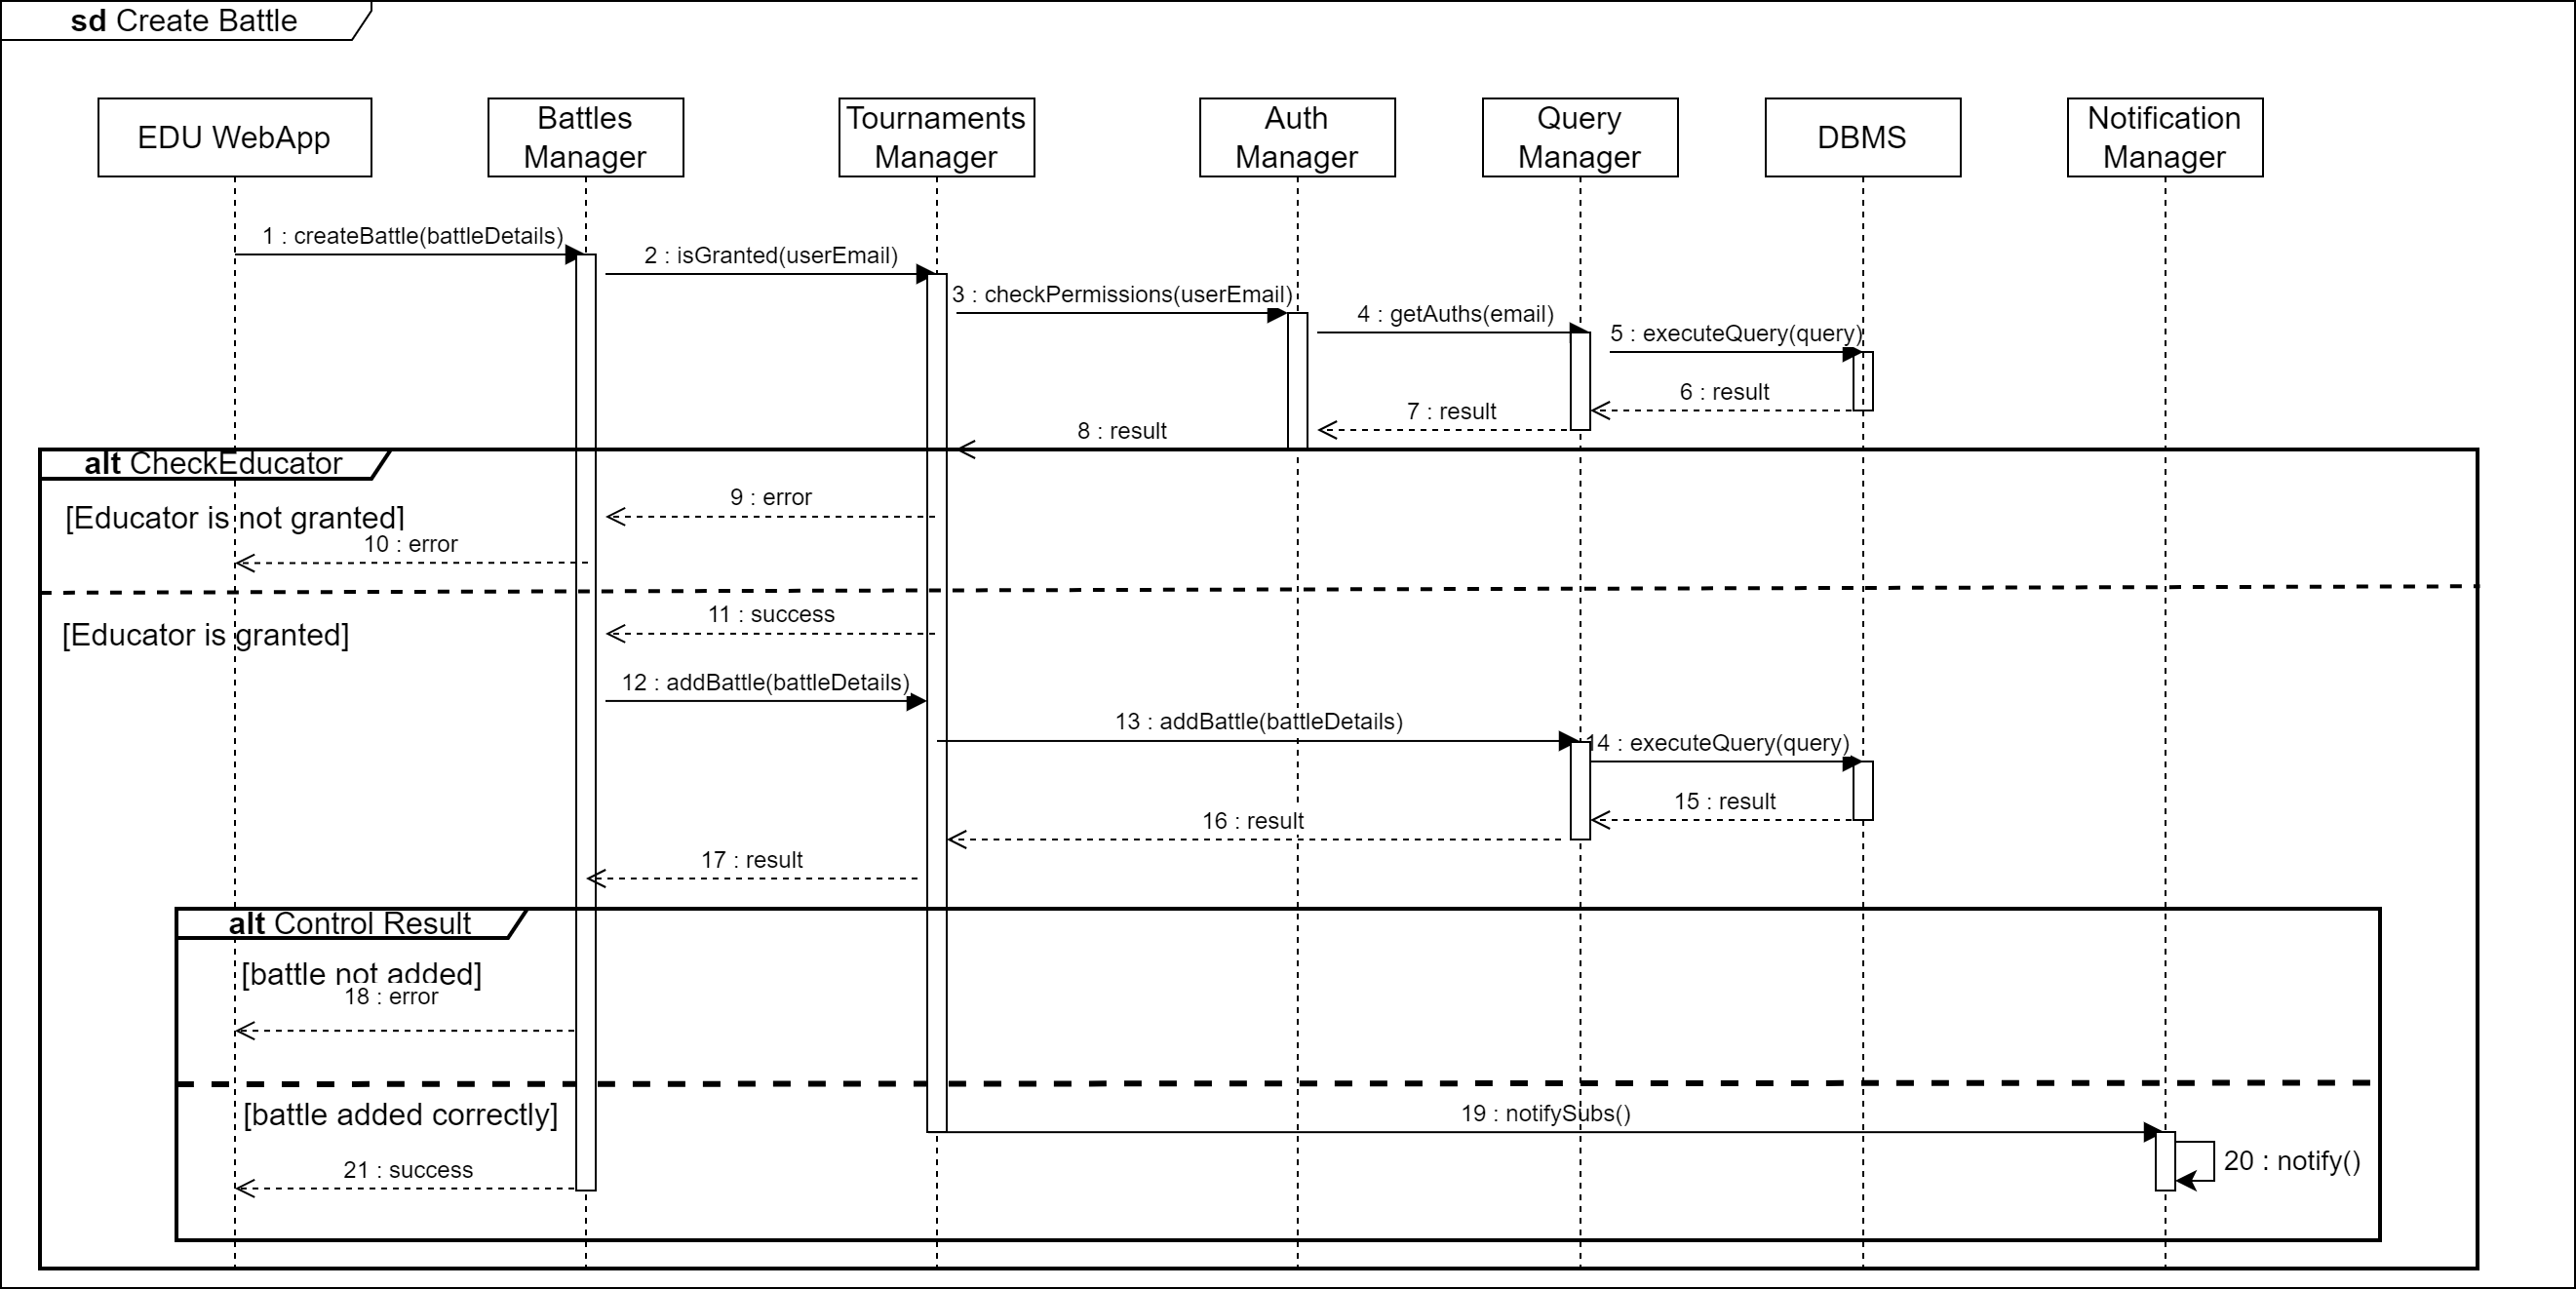
\includegraphics[width=\textwidth]{images/runtimeviews/RuntimeView_CreateBattle.png}
    \caption{Runtime View of Create a Battle Event}
    \label{fig:RuntimeView_CreateBattle}
\end{figure}

\subsection{Join a Battle Solo}
In this sequence diagram is shown how an user can subscribe to a battle. By joining the battle, the system add to the database the email of the user into the subscribed email of that battle. If the user decides to invite other members, the inserted emails are notified. (Figure \ref{fig:RuntimeView_JoinBattleSolo})
\begin{figure}[H]
    \centering
    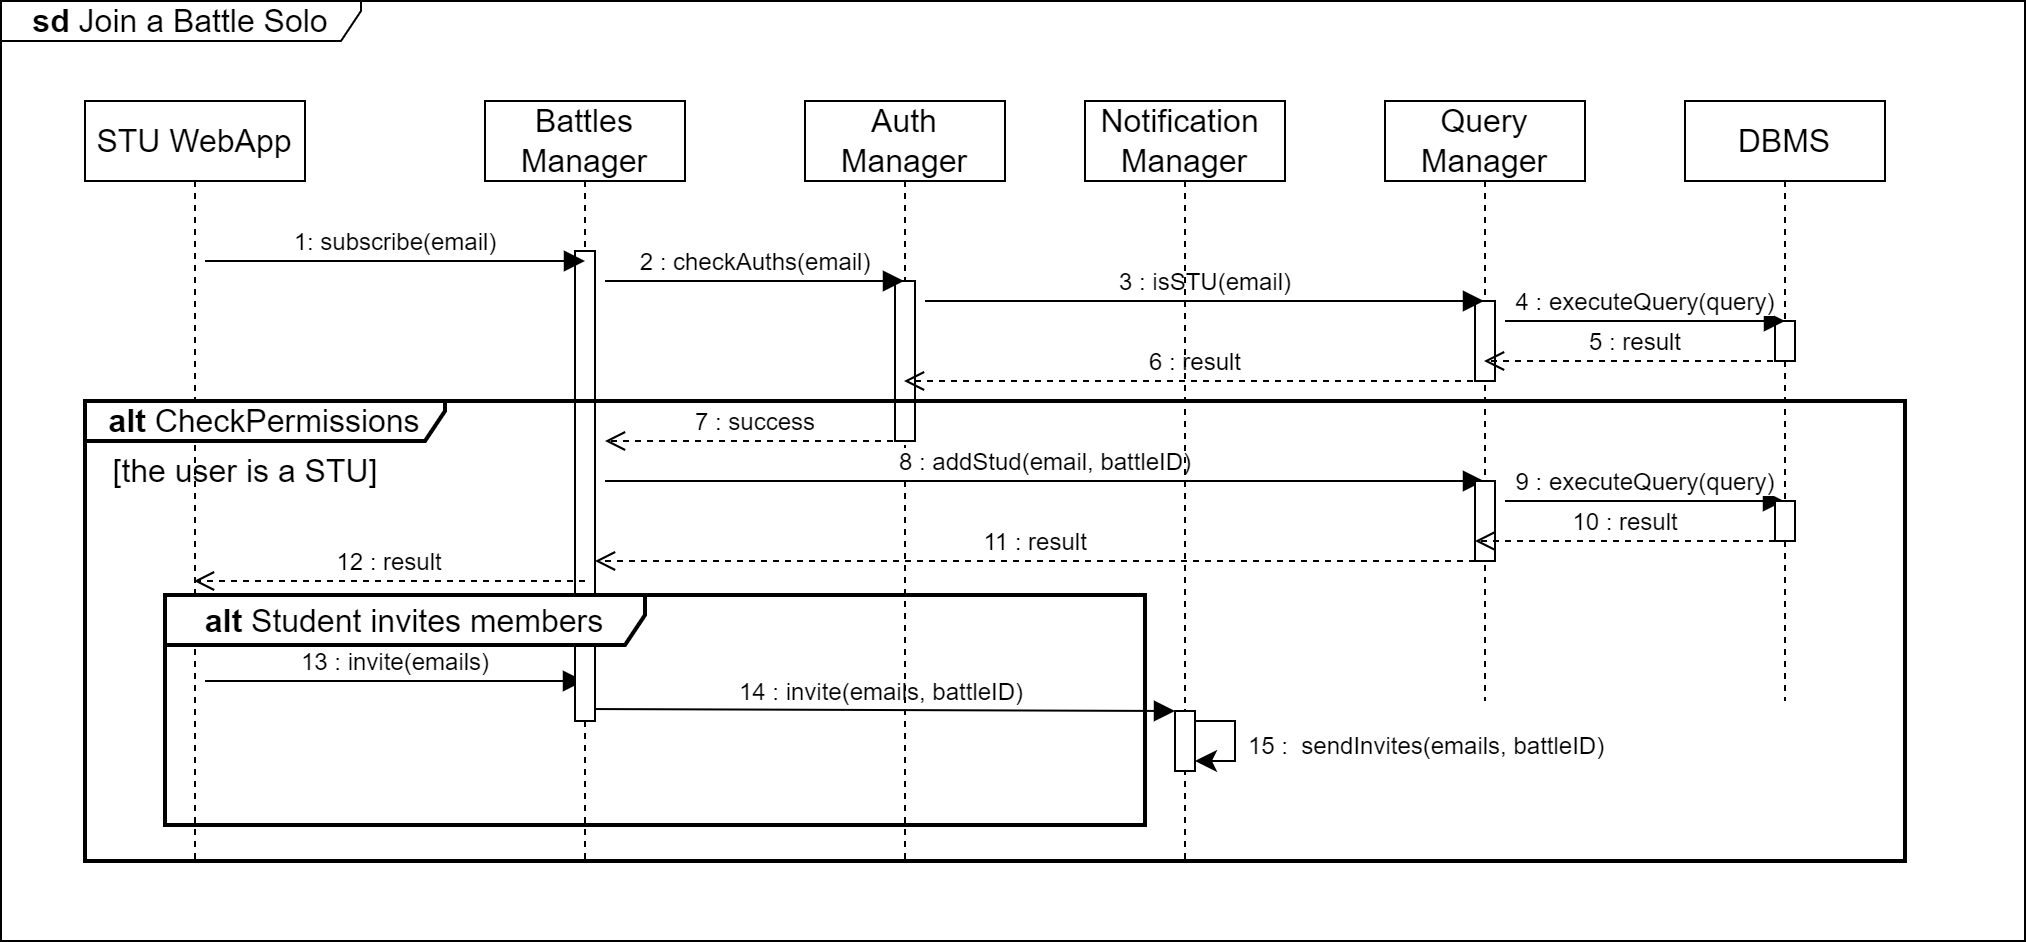
\includegraphics[width=\textwidth]{images/runtimeviews/RuntimeView_JoinBattleSolo.png}
    \caption{Runtime View of joining a Battle Solo}
    \label{fig:RuntimeView_JoinBattleSolo}
\end{figure}

\subsection{Upload code}
In this case, the GitHub API notify the system which through the related component computes the new score and update it by sending the new score to the database. Finally, the system updates the battle ranking with the new score. (Figure \ref{fig:RuntimeView_CodeUploaded})
\begin{figure}[H]
    \centering
    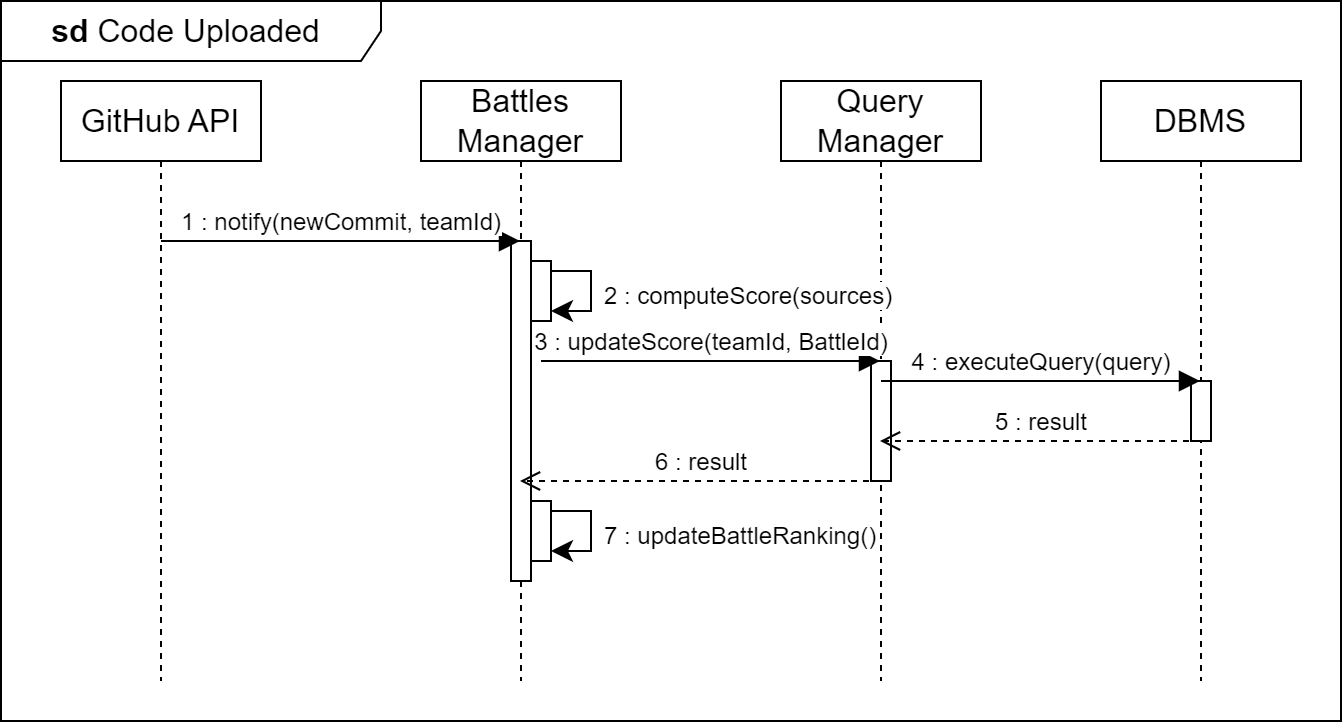
\includegraphics[width=\textwidth]{images/runtimeviews/RuntimeView_CodeUploaded.png}
    \caption{Runtime View of Notification of a new commit of a team}
    \label{fig:RuntimeView_CodeUploaded}
\end{figure}

\section{Other design decisions}
\subsection{Web Application}
As the platform's primary functionality is closely tied to coding activities, it is expected that users will predominantly employ personal computers, so there is no need to develop a mobile application, which would require a significant amount of additional work.\\
Instead, the system will be accessible through a web application, that is much easier to develop, maintain and being accessed by the users.

\subsection{Single Page Application}
The system will be developed as a Single Page Application (SPA), that is a web application that interacts with the user by dynamically rewriting the current web page with new data from the web server, instead of the default method of the browser loading entire new pages.\\
This approach will allow the system to be more responsive and to be more similar to a desktop application, since the user will not have to wait for the entire page to be reloaded every time he performs an action. Furthermore, it will allow the system to be more efficient, since the server will not have to send the entire page every time the user performs an action, but only the data that has changed, leaving the client to render the page.

\subsection{Relational Database}
We selected a relational database for our system design because it is effective at storing structured data, granting data integrity, and providing fast query performance. It can also be easily scaled to handle large amounts of data and support many concurrent users. The database allows us to store and retrieve information efficiently, while also ensuring that the data is accurate and consistent

\subsection{RESTful API}
We have chosen to implement a RESTful API for our system because it is a simple, lightweight, and flexible architecture that is easy to understand and use. It is also scalable and reliable, making it ideal for our application.\\


\chapter{User Interface Design}
Since the mockups of the user interface have already been presented in the RASD document, they are not repeated here; instead, are presented the UX diagrams.

\begin{figure}[H]
    \centering
    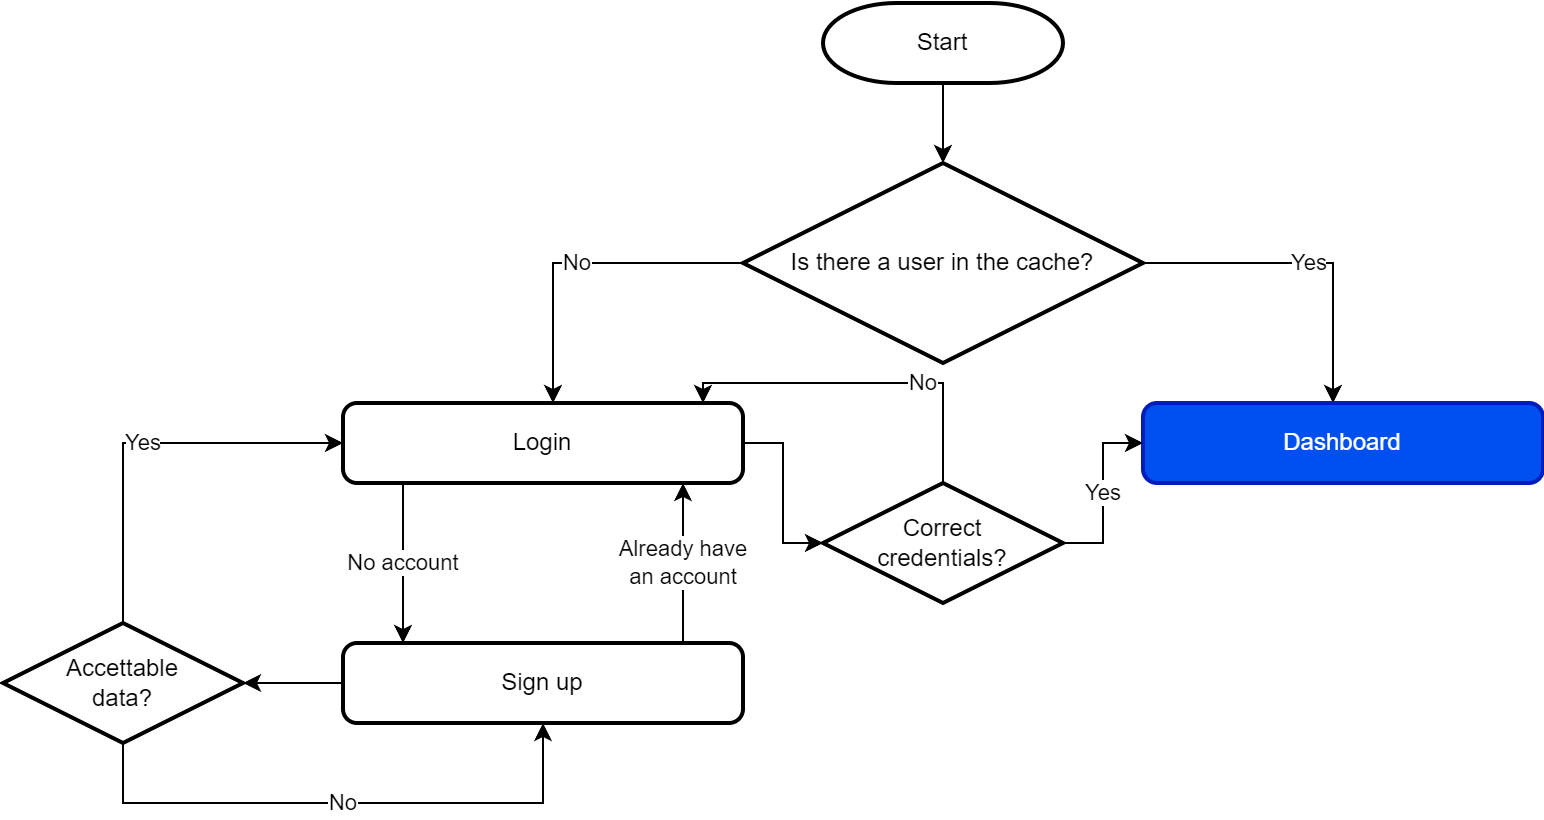
\includegraphics[width=\textwidth]{images/UX/UX-Entry_point.drawio.png}
    \caption{Undifferentiated: Entry point i.e. the login page}
\end{figure}

\begin{figure}[H]
    \centering
    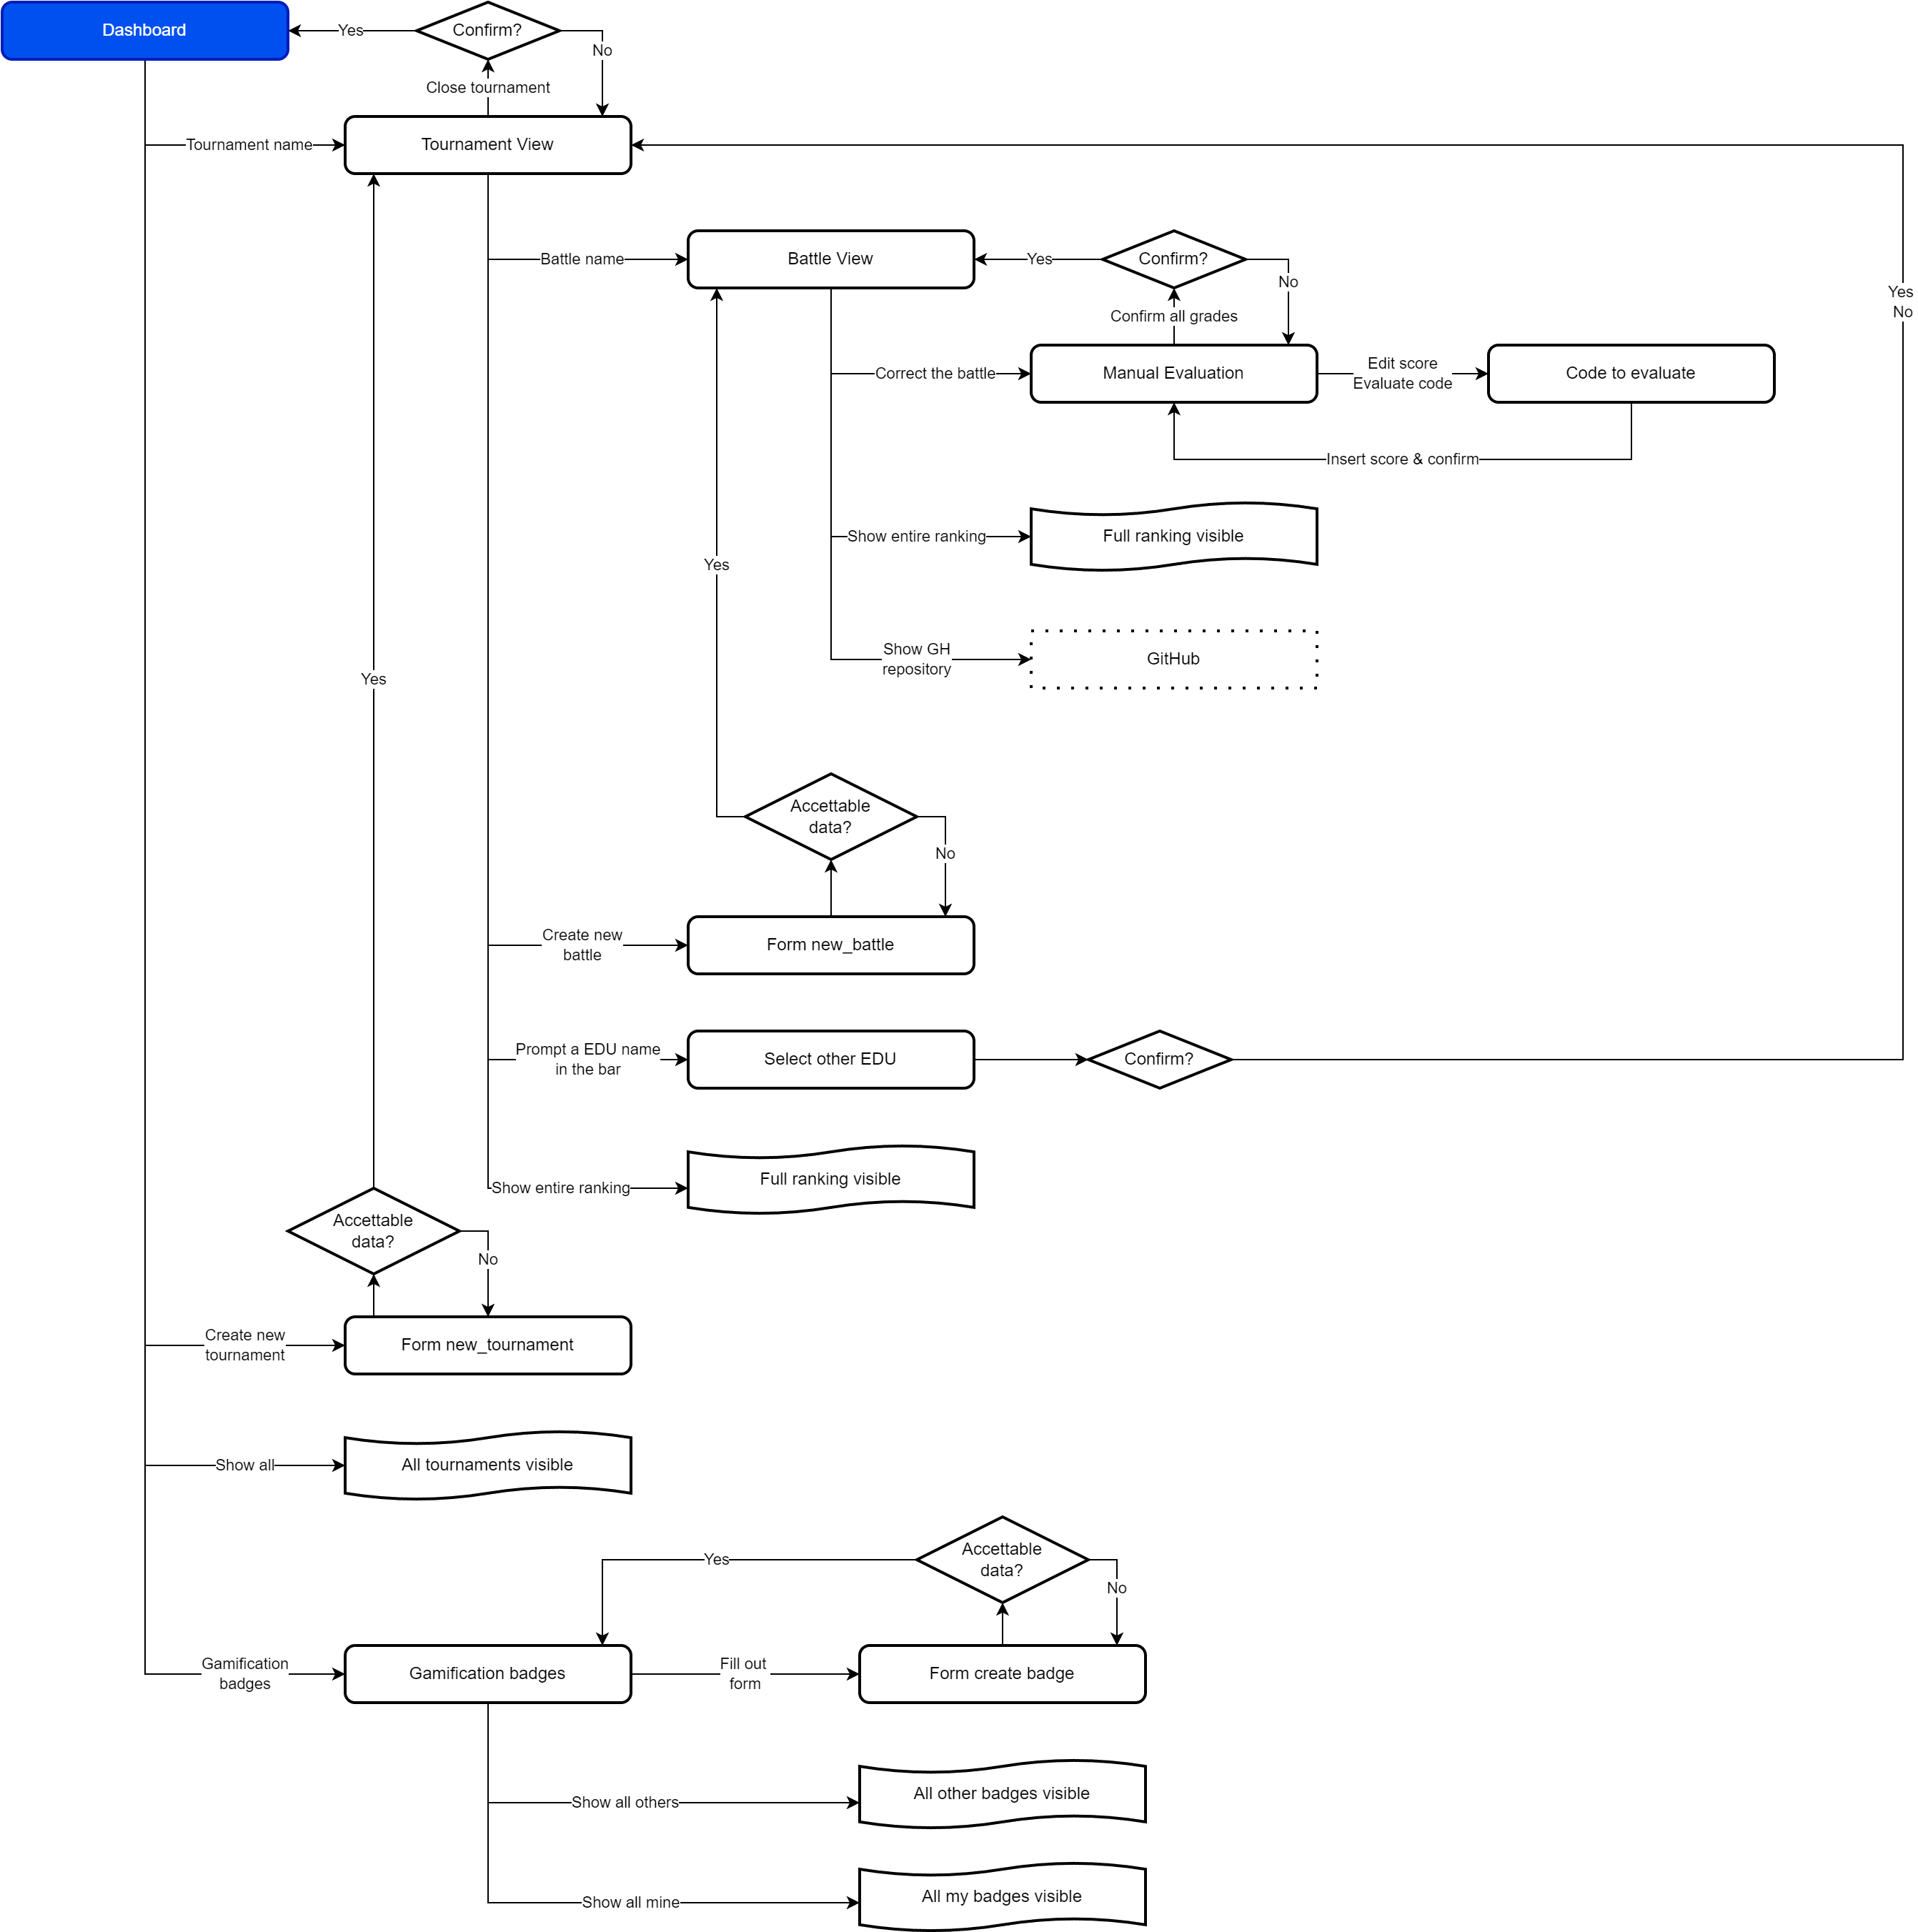
\includegraphics[width=\textwidth]{images/UX/UX-EDU.drawio.png}
    \caption{Flow graph for the EDU}
\end{figure}

\begin{figure}[H]
    \centering
    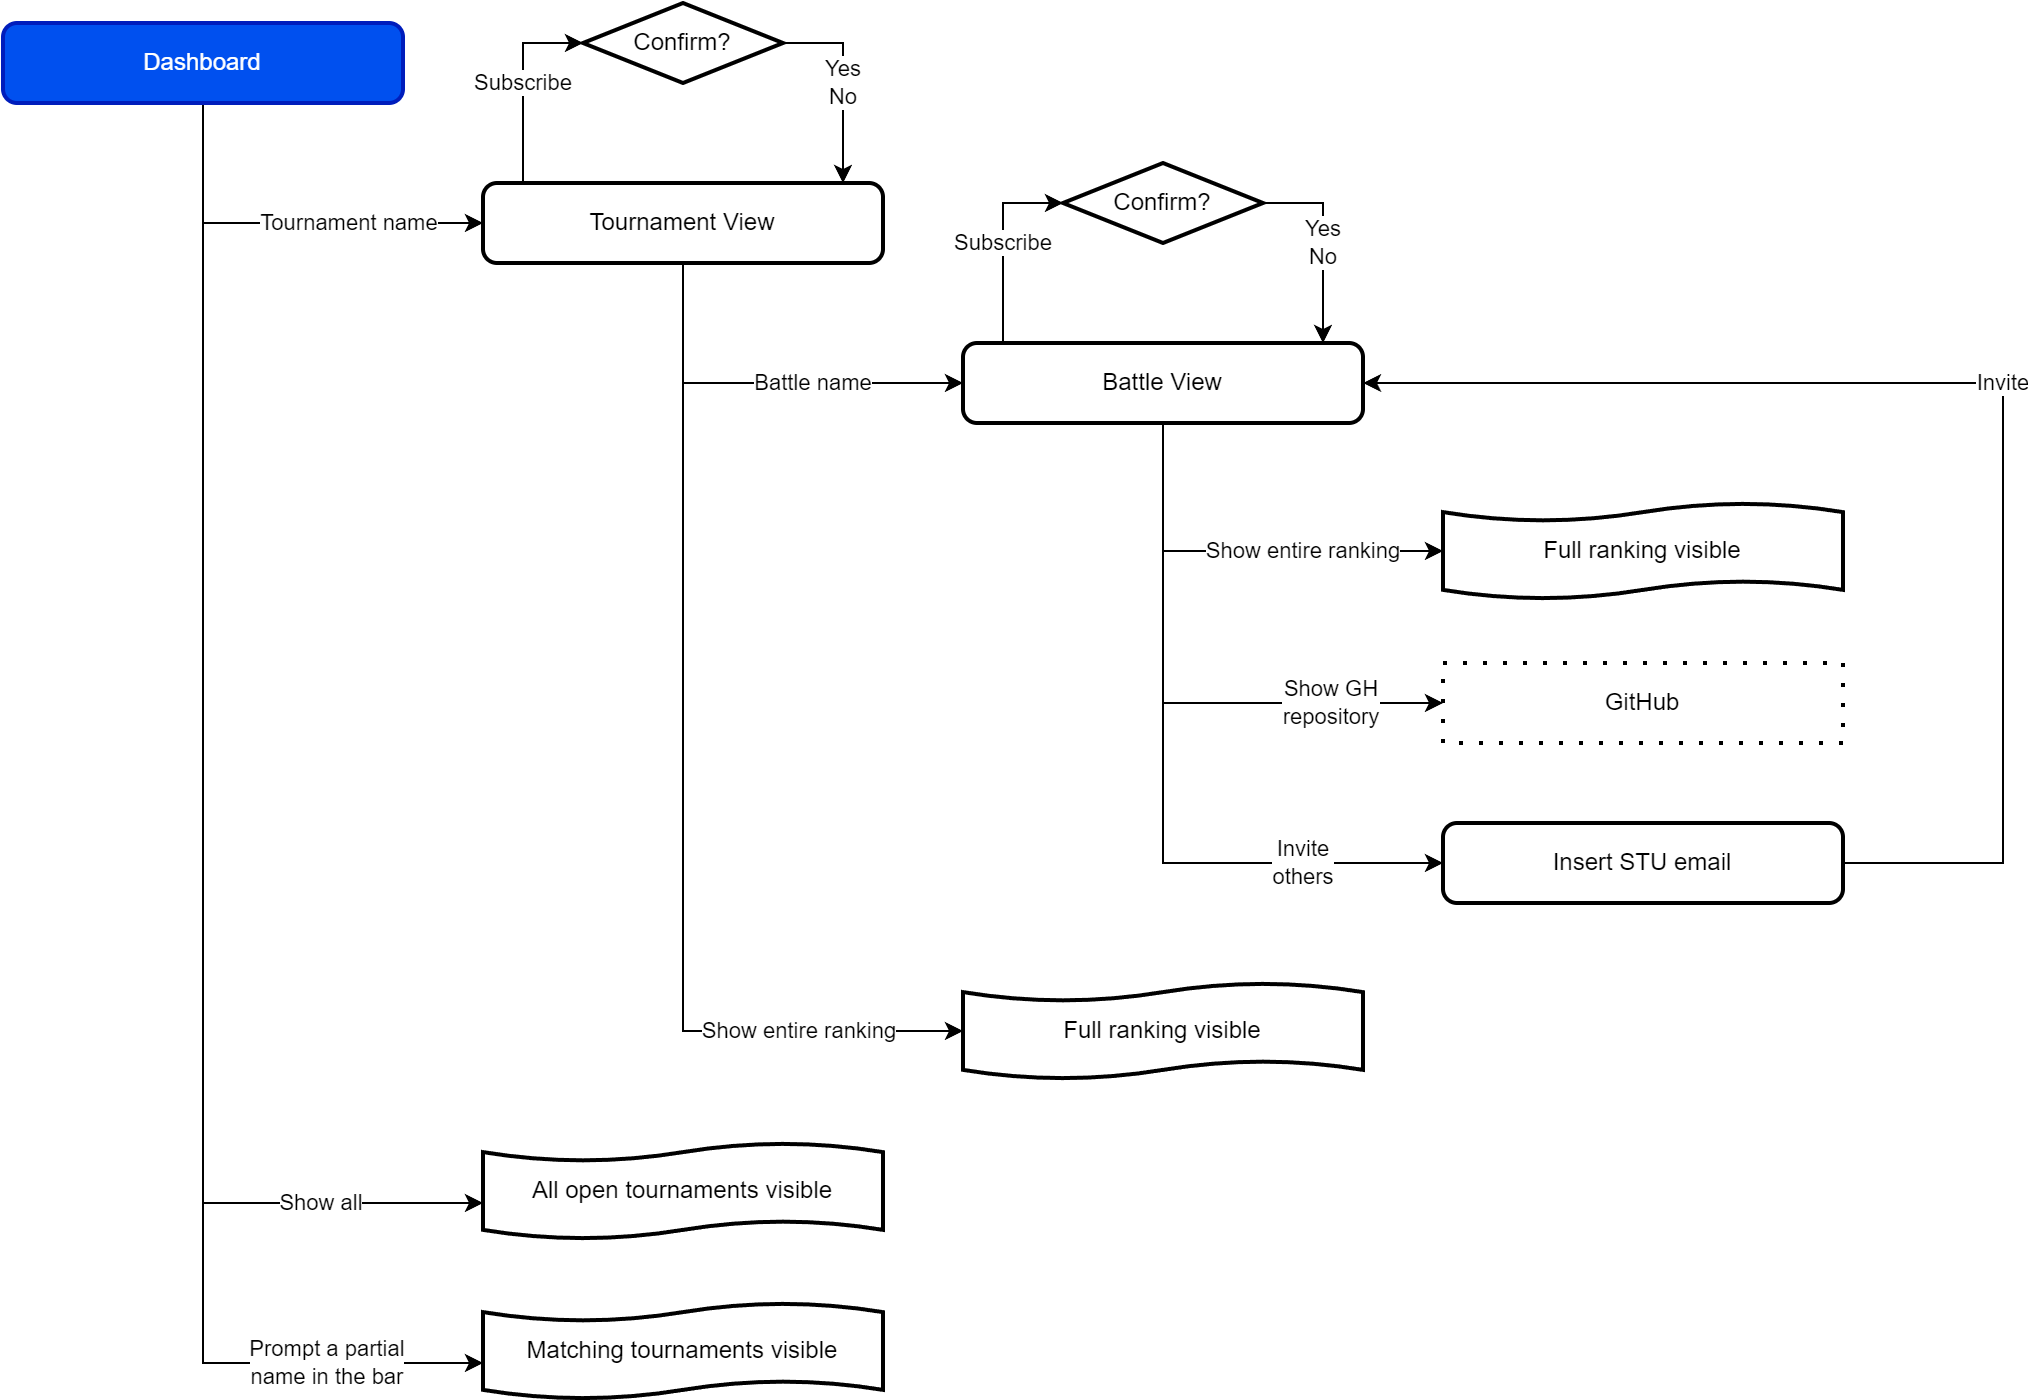
\includegraphics[width=\textwidth]{images/UX/UX-STU.drawio.png}
    \caption{Flow graph for the STU}
\end{figure}

\begin{figure}[H]
    \centering
    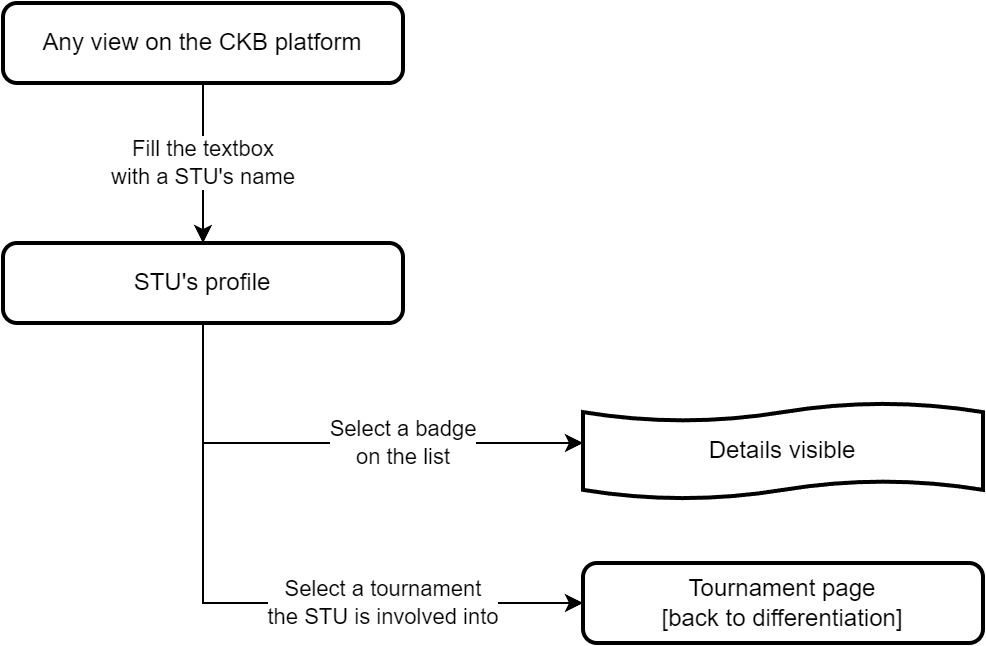
\includegraphics[width=\textwidth]{images/UX/UX-STU_profile.drawio.png}
    \caption{Undifferentiated: viewing a STU's profile}
\end{figure}
\chapter{Requirements Traceability}
ùdvwjiwv
\chapter{Implementation, Integration and Test Plan}
The application is based on three logical layers (data, logic, and presentation) that can be implemented in parallel.\\
The whole system can be tested in parallel following a bottom-up approach, this is because all the components can be developed independently and then integrated, and so the testing can be done in an incremental way to evaluate the dependencies between the subcomponents.

\section{Development plan}
Since the front-end relies on REST APIs provided by the back-end, the focus is more on the back-end development, to provide the front-end developers with the APIs needed.

\subsection{Front-end}
Even if it relies on the back-end APIs, the front-end can be developed in parallel with the back-end, since the APIs are well defined and documented.
It is sufficient to provide a mock-up of the JSON objects that will be returned by the APIs to correctly develop the front-end.

\subsection{Back-end}
Back-end development is the most important part of the project since it provides the front-end with the APIs it needs.\\
The order of development of the subcomponents is given by the dependencies between them, so the order is the following:

\begin{enumerate}
    \item \textbf{DBMS}: it is the core of the data layer, so it is the first component to be developed. It includes the implementation of the ER diagram given in Figure \ref{fig:er_diagram}
    \item \textbf{Query manager}: it is the component that provides the APIs to the logic layer that will be used to query the database. It is the second component to be developed since it relies on the DBMS and it is the only component that can access the database.
    \item \textbf{Auth manager, Notification manager}: they shall be implemented before the other subcomponents because they are used by the other subcomponents to authenticate the users and to send notifications to them. Since they are independent from each other, they can be developed in parallel.
    \item \textbf{All other subcomponents}: they can be developed in parallel since they are sufficiently independent from each other. If, for any reason, a subcomponent needs to interact with another one, it can see the other one as a black box
\end{enumerate}

\section{Integration plan}
The following section shows the order in which the subcomponents are integrated to constitute the whole system. \\
Each component must be uint tested before being integrated with the others.
The integration testing process occurs incrementally to allow for bug tracking. 
Every time a component of a dependency level is completed, it is integrated with the modules of the other levels to test the behavior of the developed subsystem. 
When the whole component is fully integrated is finally tested.\\
The order of the integration is given by the dependencies between the subcomponents, so the order is shown by the following graphs (for the sake of simplicity, the graphs show only the dependencies between the subcomponents omitting the interfaces between them):\\

The first components to integrate are the Query Manager and the DBMS since they make a connection between the application layer and the data layer. \\
\begin{figure}[H]
    \centering
    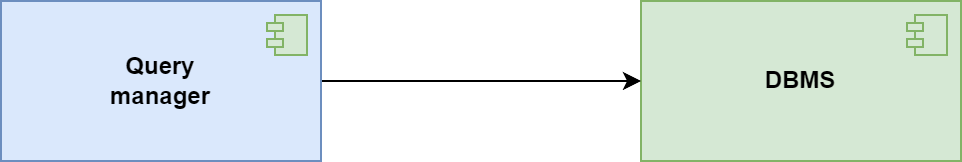
\includegraphics[width=0.6\textwidth]{images/test_plan/test-plan-1.png}
    \caption{Integration plan for the data layer}
    \label{fig:test-plan-1}
\end{figure}

The Query Manager is the only component that can access the database and nearly all the other components rely on it to query the database. \\
\begin{figure}[H]
    \centering
    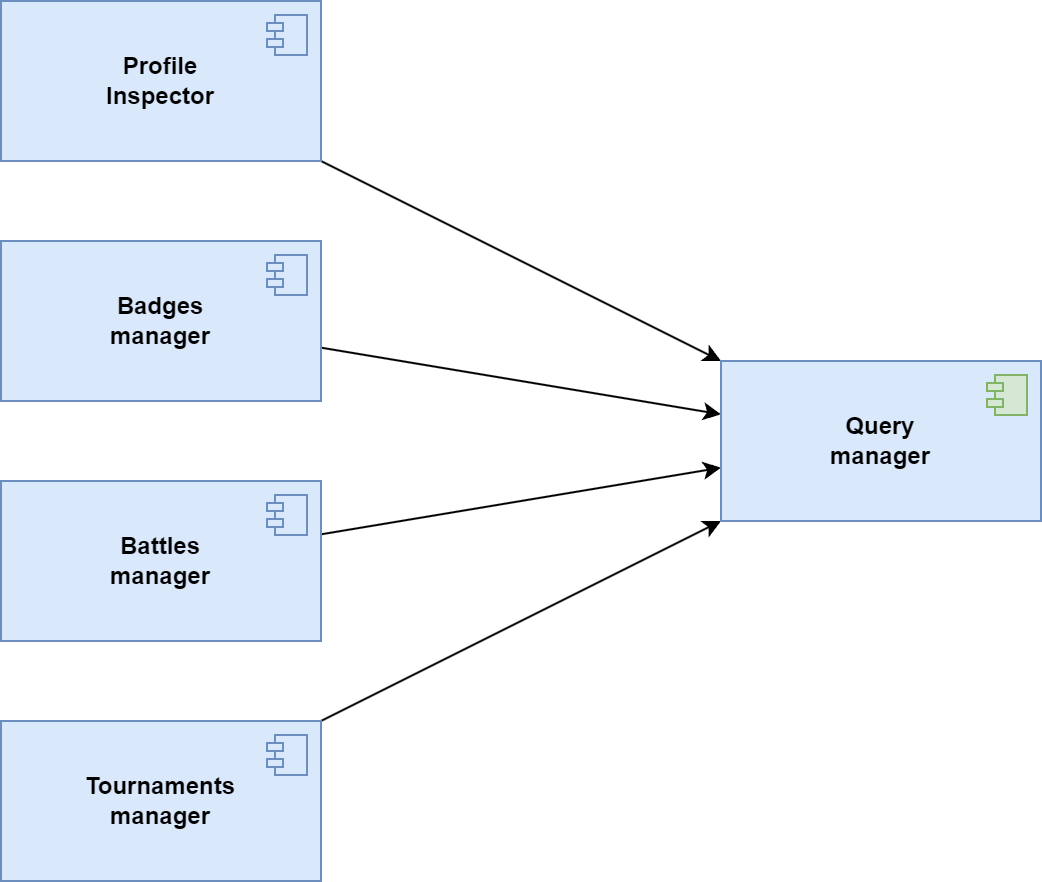
\includegraphics[width=0.6\textwidth]{images/test_plan/test-plan-3.png}
    {\color{red} Se query manager è l'unico componente che si interfaccia al DB, allora Auth Manager deve star collegato ad esso}
    \caption{Integration plan for the query manager}
    \label{fig:test-plan-3}
\end{figure}

The second component to integrate is the Auth Manager since it makes the system behave differently based on the user's permissions and so it is crucial to ensure that it works correctly before integrating other components (a concrete example is to ensure that the query to the databases are done by an authenticated user at the right level).\\
\begin{figure}[H]
    \centering
    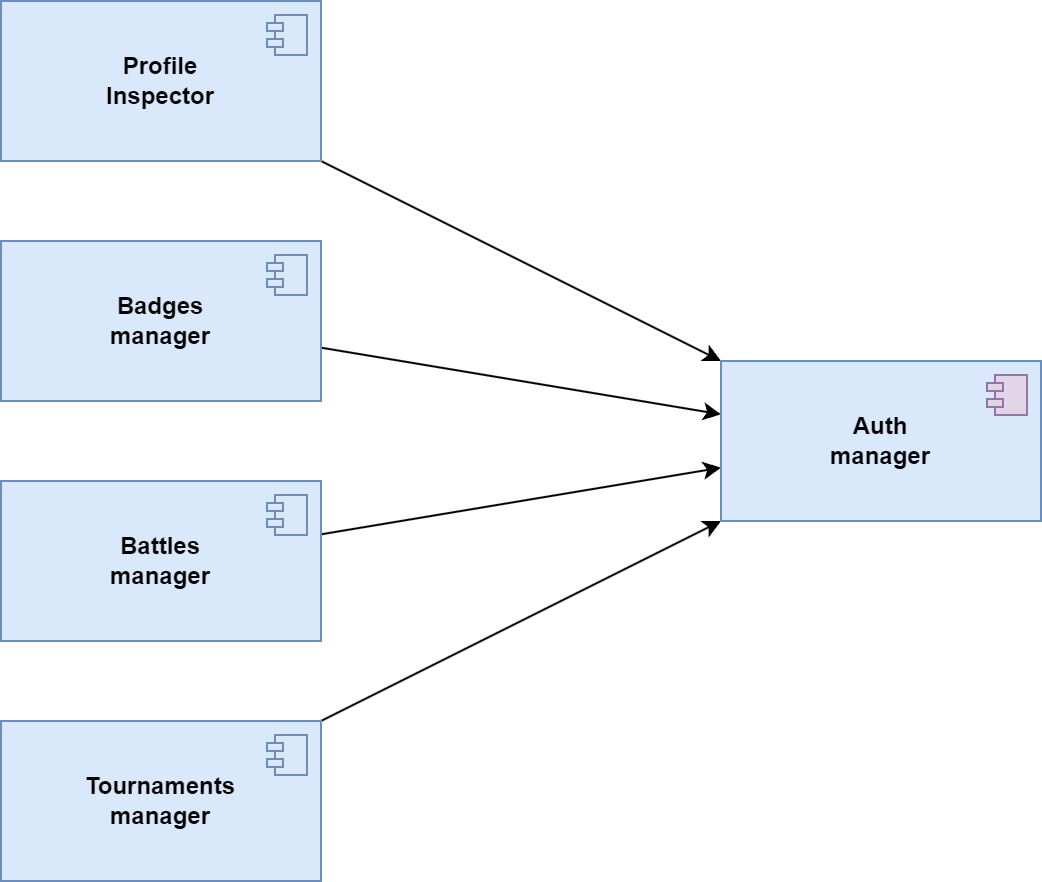
\includegraphics[width=0.6\textwidth]{images/test_plan/test-plan-2.png}
    \caption{Integration plan for the auth manager}
    \label{fig:test-plan-2}
\end{figure}

Another component to integrate is the Notification Manager, which is used to send notifications to the users. \\
It can be integrated in parallel with the Query Manager since it does not need to access the database.\\
\begin{figure}[H]
    \centering
    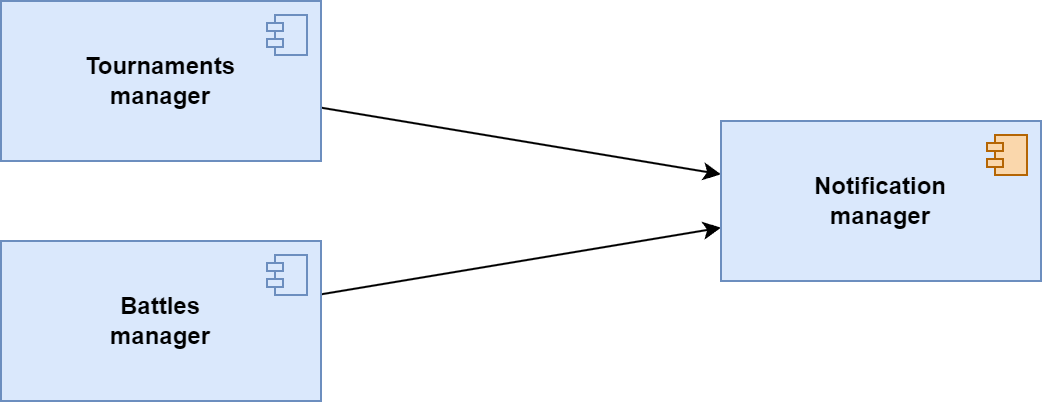
\includegraphics[width=0.6\textwidth]{images/test_plan/test-plan-4.png}
    {\color{red} Non credo si debbano mettere Profile inspector e Badges Manager}
    \caption{Integration plan for the notification manager}
    \label{fig:test-plan-4}
\end{figure}

Profile Inspector, Badge Manager, Battle Manager, and Tournament Manager are components that need to be integrated with both the Query and the Auth Manager.\\
Some of them rely on the Notification Manager as well, so they need an integration with it.\\


Finally, once all the unit tests are passed and the components are integrated, the presentation layer can be integrated with the other components and a full testing phase can be performed on the whole system.\\
\begin{figure}[H]
    \centering
    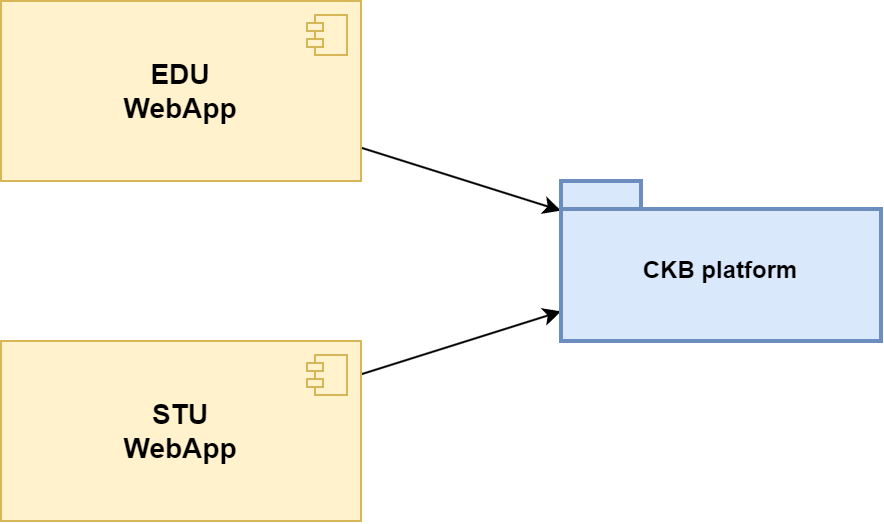
\includegraphics[width=0.6\textwidth]{images/test_plan/test-plan-5.png}
    \caption{Integration plan for the presentation layer}
    \label{fig:test-plan-5}
\end{figure}

{\color{red} Vogliamo mettere un diagramma riassuntivo di tutto l'Application server per mostrare le dipendenze?}

\section{System Testing}
The testing phase aims to verify the functional and non-functional requirements and must take place in a testing environment that is as close as possible to the production environment.\\
To ensure the minimum probability of failure of the released software, these testing performed are:
\begin{itemize}
    \item \textbf{Functional testing}: to verify that the system meets the functional requirements, in particular, the ones specified on the RASD document.
    \item \textbf{Performance testing}: to verify that the system meets the non-functional requirements, it helps to identify and eliminate performance bottlenecks affecting response time, utilization, and throughput. in particular, whether the software remains functional with increased demand and various environmental conditions.
    \item \textbf{Load testing}: to detect memory leaks, mismanagement of memory, and buffer overflows, it also identifies the maximum operating capacity of the application.
    \item \textbf{Stress testing}: to measure software robustness and error handling under heavy load conditions, it verifies stability and reliability.
\end{itemize}
\chapter{Effort Spent}

\section*{Team}

% Please add the number of hours spent for the document in this section*
% To add a new row, copy the following snippet and put it inside the table
% \description_of_the_topic & number_of_hours_spent \\ \hline

\begin{table}[H]
    \renewcommand{\arraystretch}{1.5}
    \centering
    \begin{tabular}{|l|c|}
        \hline
        \textbf{Topic} & \textbf{Time} \\ \hline
    \end{tabular}
    \caption{Effort Spent during team meetings}
    \label{tab:group-effort-spent}
\end{table}

\section*{Tommaso Pasini}
\begin{table}[H]
    \renewcommand{\arraystretch}{1.5}
    \centering
    \begin{tabular}{|l|c|}
        \hline
        \textbf{Topic} & \textbf{Time} \\ \hline
    \end{tabular}
    \caption{Effort Spent by Tommaso Pasini}
    \label{tab:pasini-effort-spent}
\end{table}

\section*{Elia Pontiggia}
\begin{table}[H]
    \renewcommand{\arraystretch}{1.5}
    \centering
    \begin{tabular}{|l|c|}
        \hline
        \textbf{Topic} & \textbf{Time} \\ \hline
        Chapter 2      & 1h30m           \\ \hline
    \end{tabular}
    \caption{Effort Spent by Elia Pontiggia}
    \label{tab:pontiggia-effort-spent}
\end{table}

\section*{Michelangelo Stasi}
\begin{table}[H]
    \renewcommand{\arraystretch}{1.5}
    \centering
    \begin{tabular}{|l|c|}
        \hline
        \textbf{Topic} & \textbf{Time} \\ \hline
    \end{tabular}
    \caption{Effort Spent by Michelangelo Stasi}
    \label{tab:stasi-effort-spent}
\end{table}


\end{document}